\documentclass[11pt]{article}
\usepackage[utf8]{inputenc}
\usepackage{amsmath,amssymb}
\usepackage{booktabs}
\usepackage{graphicx}
\usepackage{longtable}
\usepackage{array}
\usepackage[hidelinks]{hyperref}
\title{HMRS: A hierarchical management-and-retrieval system for tiered knowledge document organisation and evidence-traced access}
\author{Author Name\and Co-author Name}
\begin{document}
\maketitle
\begin{abstract}
Document collections support knowledge work only when acquisition,
organisation, maintenance and access are connected. We present HMRS, a
self-hosted system that manages collections, documents and segments through
catalogue, shelf, document and segment views. Parsed content informs collection
assignment; document files, the tree registry and per-library metadata support
lifecycle audits. An optional evidence gate scores passages without
establishing entailment; pinned search may bypass catalogue navigation.

In a 100-paper arXiv campaign, 79 were retrievable and 21 were not. A separate
400-page-per-language test measured assignment accuracy of 0.875 (English) and
1.0 (Chinese/Japanese). A scripted 72-question route audit selected the gold
collection in 72/72 full-card and 37/72 name-only cases; an unlogged fallback
may use descriptions. On the same questions, frozen annotated target-string
containment in the returned evidence pack was 52/72 for the tiered chunk-window
arm. Later executions gave 51/72 (70.8\
three records. The per-library union without catalogue navigation (PD) reached
45/72, with the difference unresolved, and a scoped flat union reached 39/72.
A target string may occur in a sibling document, so these are lexical
 evidence-pack proxies, not gold-document retrieval or semantic answer quality.
Arms
vary in multiple components; the flat lookup
may depend on the gold domain. Gold identifiers appeared in all 60 answer-or-
trace cells. Because an identifier in a trace need not have been read, this
check does not establish document reachability; document-style citation markers
separated the arms (9/10 versus 2/10), a lexical contrast, not semantic
quality. In a same-pool replay of a retired hybrid wrapper, verifier
re-ranking lowered Hit@5 from 15/16 to 7/16;
fusion order restored 15/16. All 191 recorded scores exceeded threshold.

The results document an auditable structure, not general retrieval superiority,
semantic answer quality or reliability. This replay warns against one
historical ordering configuration; filtering was not tested on that pool.
\end{abstract}

\noindent\textbf{Keywords:} Knowledge document management · Document classification · Hierarchical organisation · Tiered retrieval · Evidence verification · Model Context Protocol

\vspace{1em}

\section{Introduction}


Enterprises record regulations, failure analyses and operational lessons in
unstructured documents. Using such documents as a knowledge base requires
reliable parsing, placement in appropriate collections and attention to
consistency as those collections change.
A query may need to move from the relevant collection to a document and then
to the passage that carries the evidence, while retaining a pointer to its
source.

These requirements span document management and query-time retrieval.
Modular RAG and retrieval surveys already treat indexing and pre-retrieval as
pipeline modules [1,2]; this study examines how
collection placement, lifecycle operations and per-tier audits connect to the
retrieval step that consumes that state. In retrieval-augmented generation
(RAG), retrieved material informs generation; dense retrieval can embed queries
and passages in a shared vector space [3,4]. Agentic systems let a language
model call retrieval tools [5,6], and hybrid, lexical
and graph-structured variants extend the ranking model
[7--11]. Knowledge management
addresses the collection itself: enterprise content management governs
organisational documents [12,13],
metadata and tagging studies ask how documents are described and reviewed
[14,15], and public knowledge
bases curate facts under explicit ontologies
[16,17]. Semantic similarity
measures topical relatedness rather than evidence containment, a failure mode
discussed in the hallucination and RAG surveys [2,18].
A relevant passage may remain hard to reach if its collection was not
properly classified, its description does not reflect its content, or a
rename left the index stale.

The management--retrieval boundary creates a systems problem: an index alone
cannot ensure that a query reaches an appropriate collection, document and
passage. Distributed information retrieval has long studied collection
selection [19,20]. This work connects selection
to managed collection state and audits selected lifecycle outcomes. It asks how
a document collection can be managed so that a query can proceed from
collection to document to segment, with each transition open to inspection.
We study this question through an implemented system and bounded operational
audits. Integration by itself is not treated as evidence of improved retrieval
or answer quality.

HMRS (Hierarchical Management Retrieval System) is a self-hosted
knowledge document management system. It maintains collections, documents and
segments and supports catalogue, shelf, document and segment views. In the
catalogue-first policy, the catalogue exposes collection descriptions, the
shelf exposes document descriptions within a selected collection, the document
view opens its body, and the segment view exposes indexed passages. Pinned
search can bypass catalogue and shelf selection; these are access views over
the managed objects, not four separate storage levels. An ingest agent selects
collections from parsed content, while lifecycle audits compare document files,
tree-registry entries and per-library metadata. The optional evidence gate
scores candidate segments; it does not prove support. Answer workflows
distinguish a completed search without evidence from tool failure. These
stages are described in Sections~3--7.

The platform integrates document parsing, content-informed collection assignment,
content-derived descriptions and tags, lifecycle management, the tiered access
path and a Model Context Protocol (MCP) server [5]. It runs locally and
exposes management and retrieval functions to several agent harnesses. We
distinguish implemented functions from those exercised by the reported
campaigns: the paper evaluates the management loop first, then examines how
access workflows use the managed state to retrieve evidence.

\noindent\textbf{Contributions.}
\begin{enumerate}
\item A management--retrieval contract for knowledge documents. HMRS represents
collections, documents and segments as managed objects and connects parsing,
content-informed placement, descriptions/tags, lifecycle updates, indexing and
catalogue-first access through one auditable state. It compares document files,
the tree registry and per-library metadata after selected operations, and
distinguishes checks enforced by tools from semantic decisions made by agent
workflows (Sections~3--7).
\item A collection-assignment and route-card audit. In a 100-paper arXiv
campaign, 79 papers were retrievable and 21 were not, with incomplete failure
attribution. In a separate ingestion test on 400 Wikipedia pages per language,
content-based assignment accuracy was 0.875 for English and 1.0 for Chinese and
Japanese. In a 72-question scripted audit, full route cards returned the gold
collection for 72/72 questions, compared with 37/72 for nominally name-only
cards. An unlogged fallback could still use descriptions, so this is a
configuration contrast, not an isolated treatment effect
(Sections~8.4 and~8.2).
\item A bounded content- and answer-layer account. Six evidence
configurations are compared on one fixed question set: A0 is the tiered
baseline; A0f reads full document windows; A0h additionally unions vector
chunk windows; PD is a navigation-free per-library union; A1b is a scoped
flat vector union; A2 drops the evidence gate (configurations defined in
Section~8.6). On the same 72 questions,
the latest complete same-question follow-up (the R3 record) contained the
annotated target string somewhere in the returned evidence pack in 51/72 cases
for A0h, compared with 45/72 for the per-library union without catalogue
navigation (PD), 44/72 for A0f, 39/72 for A0 and A1b, and 25/72 for A2. A
sibling-document occurrence may count; these are lexical proxies, not
gold-document retrieval or semantic answer correctness. The frozen A0h result
was 52/72, and A0h
was the highest configuration in the frozen run, an archived reproduction
and the follow-up, with the A0h $>$ PD $>$ A0f ordering preserved and no
per-question flips for A1b and A2. The A0h--A0 contrasts were 15--0 frozen
and 12--0 in R3 ($p=6.1\times10^{-5}$ and $p=0.00049$, unadjusted). The arms
vary in multiple components and the flat lookup may depend on the gold
domain. A mechanical
full-read script found the strings in 72/72 cases after reading 879 parts, but
generated no answers; the R3 read-all run was incomplete. Separately, two
ten-question answer grids reported gold identifiers in the answer or trace for
all 60 cells. Because a trace identifier need not have been read, this check
cannot establish document reachability; document-style citation markers
separated the arms (9/7/2, and 9/9/9 on a common substrate). These lexical
checks do not establish semantic correctness or claim-to-source support
(Sections~8.6 and~8.7).
\item A same-pool diagnostic of verifier role. In a replay of a retired hybrid
wrapper, verifier-score ordering reduced Hit@5 from 0.94 to 0.44, while retaining
fusion order restored 0.94. All 191 recorded scores exceeded the configured
threshold, so filtering did not activate and remains untested on this pool
(Sections~6 and~8.9).
\end{enumerate}

\subsection{Research questions and reading guide}


Five questions connect the management model to the evidence and keep each
conclusion within the scope of its measurement. \textbf{RQ1} asks whether
documents can be parsed, automatically classified into a collection and stored
with state that stays consistent across the three sources, and where that
process fails. \textbf{RQ2} asks whether the tiered path selects the correct
collection and narrows to the documents that contain the target evidence, and
what the collection-selection contrast does and does not establish.
\textbf{RQ3} compares the tested content-layer configurations on
annotated target-string containment in returned evidence packs and retrieval
cost on the same question corpus, and asks whether the tiered path contains
more of this lexical proxy than flat or navigation-free alternatives.
\textbf{RQ4} examines
how verifier-score ordering affects recall and what can be inferred about
filtering when the configured threshold rejects no recorded score.
\textbf{RQ5} summarises observed abstention, runtime, tool cost and execution
failures at the answer layer.

Section~2 positions the work; Sections~3--
6 describe the management model, the collection and
document levels, and the tiered access path;
Section~7 covers deployment and enforcement; and
Section~8 evaluates the system, followed by implications,
limitations and conclusions in
Sections~9--11.


\section{Related work}


\subsection{Knowledge management and document acquisition}
Studies of LLM integration with knowledge-based methods describe both the
potential and the challenges of combining language models with structured
knowledge [21]. Public knowledge bases organise facts under explicit ontologies
[16,17], whereas enterprise content
management emphasises governance over organisational documents
[12,13]. Research on organisational
knowledge explains how tacit experience becomes shareable
[22,23]; adjacent work studies metadata
quality, tagging, human review and auditability
[14,15,24,25]; automated text categorization provides the classification backbone [26]. These strands motivate reliable placement
and governance, but do not by themselves connect those controls to evidence-
checked answers. Document-AI methods, including layout-aware analysis and
MinerU, recover text and structure from complex documents
[27--29]. Near-
duplicate detection and provenance provide complementary safeguards during
ingestion [30--32].
HMRS treats acquisition quality, automatic classification and traceable
indexing as design commitments to be tested rather than as preprocessing
assumptions; the campaigns measure where they hold and where they fail,
without establishing a causal link to answer quality.

A line of work in this journal takes an explicitly architectural form: a
software reference architecture for journalistic knowledge platforms is
derived from the literature and a prototype, specifying module
responsibilities and architecture principles [33], and an
earlier workshop version outlines the architecture and a proof-of-concept
[34]. Other work builds and evaluates complete
knowledge-grounded systems---dialogue systems with graph-based semantic
models [35], OpenQA systems for low-resource languages
[36], an LLM-based clinical decision support system
[37], and an IR system for bank supervisors
[38]---while privacy-preserving service frameworks
[39] and LLM-assisted construction of expert systems
[40] treat deployment constraints as design inputs.
Domain knowledge bases are built either from operator--function descriptions
[41] or by instantiating ontologies with LLM-generated domain
knowledge [42]. The same systems orientation appears in an
open-source multi-agent framework for evidence-based knowledge-graph enrichment
[43], LLM-agent systems for data-driven engineering
modelling [44], end-to-end LLM systems for circuit analysis
[45], and an intelligent system that automates
hyperparameter tuning for gradient-boosted trees [46].
HMRS shares this systems orientation but
makes collection membership, derived descriptions and lifecycle state the
auditable objects, rather than proposing a reference architecture or a domain
ontology.

\subsection{Retrieval, organisation and agentic search}
RAG grounds generated responses in retrieved passages [3]; dense
retrievers learn shared query--passage representations [4], while BM25
remains a strong lexical baseline [7]. Ghali et al. combine
semantic retrieval, vector storage and language models to query structured and
unstructured data [47]. Hybrid retrieval combines
sparse and dense signals, including reciprocal-rank fusion
[8]; embedding models such as BGE-M3 support multilingual and
multi-granularity search [48]. Graph- and tree-structured systems
organise and retrieve structured relationships: GraphRAG adds entity-relation
graphs and community summaries [9], LightRAG uses dual-level
retrieval with incremental graph merging [10], and RAPTOR builds a
recursive cluster tree [11]. RMR-SST represents multimodal
engineering-document content as structured semantic trees and retrieves
across abstraction levels [49]. Hierarchical
representation is therefore already an established retrieval concern: RAPTOR summarises a tree of clusters over
document text and retrieves over that tree, and GraphRAG retrieves over an
entity graph induced from the corpus. HMRS differs in what the hierarchy
governs. Its hierarchy is a management structure over collections and
documents---which collection exists, which document belongs to it, which
description explains it---and selected lifecycle outcomes can be audited
across its state sources. The original RAPTOR and GraphRAG formulations build these hierarchies
offline at index time---recursive cluster summarisation and pre-generated
community summaries, respectively [9,11]. LightRAG
does contribute incremental graph updates [10], so HMRS's
difference is not incremental update per se but the governance of collection
membership and document lifecycle, reconciled across three state sources.
Incremental vector-index maintenance is itself an
active systems concern [50,51]; HMRS
complements it at the metadata layer with an explicit re-index operation and
three-source reconciliation. Retrieval granularity is likewise a design
variable: proposition-level and late-chunking strategies change what a
retrievable unit carries [52,53]. TEIE-RAG
combines hierarchical semantic chunking with retrieval-model tuning and source
grounding for engineering information extraction [54].
HMRS splits at recognised structural markers and indexes the resulting parts.
HMRS uses a
narrower document--library--tag graph for navigation and candidate
expansion; the graph does not establish answer evidence on its own.

The decision of which collection to consult has a longer history in
distributed IR: resource-selection methods such as CORI and ReDDE rank
collections by estimated relevance before searching within them
[19,20]. HMRS adopts the same
select-then-search ordering but treats collections as managed, reconciled
state rather than static statistical summaries.

Tool-using agents extend retrieval through iterative interaction
[55,56]. MCP standardises access to tool servers
[5], while Modular RAG and agentic-retrieval surveys describe
reconfigurable retrieval pipelines and their efficiency challenges
[1,6]. DeepRead performs structure-aware
reasoning for agentic search: it converts a document to structured Markdown,
indexes paragraphs with section coordinates, and lets an agent locate then
read sections in order [57]. Its hierarchy is thus a read-only,
per-document navigation aid built once at ingestion. HMRS differs in scope
and in lifecycle: its hierarchy spans collections and documents, is a
persistent managed asset whose state can be audited after selected operations, and exposes the
catalogue-first librarian lane alongside dense and hybrid alternatives under
explicit call and tool policies.

Recent articles in this venue extend the retrieval stack in complementary
directions: retrieval-augmented generation over engineering design knowledge
[58], soft-prompt tuning of dense retrievers
[59], and an evaluation of semantic-relation query expansion
in retrieval systems [60]. Private-library retrieval
supports code generation [61]; work on knowledge graphs
ranges from studying how LLMs comprehend graph facts supplied in different
prompt formats [62] to prompting LLMs with graphs for
long-tail factual questions [63], while fine-grained
stateful exploration navigates graphs through an LLM [64].
Real-time financial data grounding [65] and coordinated
multi-agent answer generation [66] illustrate the
range of deployed configurations. These systems optimise what is retrieved
and how it is used; HMRS instead asks which managed collection is
authoritative and whether its state can be audited after each lifecycle
operation.

\subsection{Verification, correction and abstention}
Two further lines border the design without competing with it. Agent memory
systems treat memory as an agent-managed store of interaction records:
MemGPT pages memory between a context window and an external store
[67], Mem0 extracts and consolidates long-term memory from
conversations [68], and A-MEM organises notes as an agentic memory
graph [69]; continual-learning work adds an information-theoretic dual
memory system [70]. HMRS manages a document corpus with audited lifecycle
state; the stores are complementary rather than competing, and an ingest
agent of the kind these frameworks assume can also use collection assignment
and consistency checks of the kind examined here. Knowledge organisation
standards such as SKOS [71] and Dublin Core provide conventions for
vocabularies and descriptive metadata; HMRS derives collection and document
descriptions from parsed content at ingest time.

Self-RAG and CRAG integrate evidence assessment or retrieval correction into
generation [72,73]; FLARE triggers retrieval during generation
[74]. Selective prediction under domain shift [75],
identifying what LLMs do not know [76,77],
ontology-grounded retrieval [78], and citation verifiability
[79,80] address adjacent concerns. EPRAG
diagnoses evidence states to choose responses, clarification or abstention in
multi-source enterprise retrieval [81]. HMRS externalises
verification as a reusable server-side operation: the gate fetches document
text, judges evidence and returns provenance to the answer layer. This design
makes the verifier inspectable, but not infallible.

The LLM-as-a-judge literature documents preference bias, imperfect agreement,
listwise instability and self-preference [82--84]; outcome-based verification can reward flawed reasoning
[85]. These findings motivate separating evidence
verification from rank ordering and testing abstention at the answer layer.

Trustworthiness and evaluation are also studied at the systems level in this
venue: a systematic meta-survey of explainable AI [86],
logic-grounded metamorphic testing of reasoning reliability
[87], and a benchmark plus evaluation framework for multi-step
clinical diagnosis [88]. These contributions supply the
vocabulary of reliability and graded evaluation; the distinction claimed here
is narrower: HMRS reports the measured failure mode of its own evidence gate
and turns that negative result into a configuration rule.

\subsection{Research gap}


Supplementary Table S11 compares representative strands rather than every
system in the literature. Prior work already studies selective question
answering, citation verifiability and retrieval correction; the distinction
here is not that abstention or evidence checks are absent from prior research.
The gap this study addresses is therefore a systems question: how can a
knowledge-document platform make the management state that precedes retrieval
observable, maintainable and usable by an agent? HMRS examines the complete
workflow from acquisition checks and automatic collection assignment through
three-source consistency, lifecycle operations, catalogue-first access and
answer-time evidence inspection. It reports where implementation and transport
boundaries constrain the workflow and measures verifier admission separately
from verifier ordering. The contribution is an auditable management--retrieval
contract, not a claim that prior systems lack reusable verification or that one
retrieval algorithm is universally superior.

The study treats three design commitments as questions to test: whether
content-based classification and lifecycle checks expose collection state;
whether a retrieved document should be re-ranked by a verifier or retain its
fusion order; and whether agent workflows can report absence while separating
completed negative searches from execution failures. Its contribution is a
knowledge document management workflow that connects and exposes stages from
parse admission through answer-evidence reporting, a per-question account of
answer-layer checks, and a same-pool diagnostic showing a loss under verifier-score ordering
when the tested threshold admitted every recorded score. It
proposes no new ranking algorithm and does not claim that the underlying
retrieval problem is solved.


\section{System overview and management model}


HMRS is a self-hosted knowledge document management system for converting
heterogeneous documents into managed, searchable collections. A Python
parsing service, a TypeScript web application and an MCP tool server share
local storage and retrieval engines [5]. The design follows from the
dependency chain of Section~1: what a document is parsed as
determines what can be indexed, the collection it is filed into determines
which tier can see it, and the tiers that follow determine whether a
supporting passage is ever read. The primary object of the design is therefore
the managed collection rather than the query. State is made auditable through
three sources---the document files, the tree registry and per-library
metadata---so that a management operation can be checked against what it
claimed to do. Each check belongs to the platform operation or calling
workflow that performs it, and the evaluation reports evidence at that level.

\subsection{Management levels and the tiered access path}


The access path has four views over three managed object levels. The catalogue
view exposes collections and their descriptions; the shelf view exposes
(document, description) entries within a selected collection; the document view
opens a document body; and the segment view exposes indexed parts and, when
invoked, their evidence scores and provenance. The shelf is a listing view, not
a fourth storage level, and a pinned search may bypass catalogue and shelf
selection. The levels describe maintained objects and operations; the views
describe what a query or agent can inspect and in what order.

\begin{table}
\centering
\small
\setlength{\tabcolsep}{4pt}
\renewcommand{\arraystretch}{1.15}
\caption{Management levels and the tiered access path. Each level names the
objects it maintains, the operations that write them, the state that describes
them, the tier that reads them, and the measurement that exercises it.
The selected access policy determines which tiers are visited; a pinned
search can bypass catalogue navigation.}

\begin{tabular}{@{}p{4cm}p{4cm}p{4cm}p{4cm}p{4cm}p{4cm}@{}}
\toprule
Level & Objects and operations & State description & Read tier & Check & Evidence\\
\midrule
Collection & libraries and sub-libraries; automatic assignment from parsed content; description and tag derivation; catalogue listing & library registry, per-library metadata, library-level index & catalogue & catalogue inventory and description round-trip & E1, E2\\
Document & documents and their parts; duplicate review; move, rename, delete; forced re-index & document files, tree registry, per-library metadata & shelf & reconciliation on selected operations & E2\\
Segment & structural split; dense and lexical indices; optional evidence gate & chunk identifiers, per-segment scores with provenance & document and segment & index coverage and post-index probe & E1, E5--E9\\
\bottomrule
\end{tabular}
\end{table}

At the collection level an ingest agent can classify a parsed document against
the catalogue of library descriptions and select a collection based on its
subject. The same workflow derives descriptions and tags from the body rather
than the filename; these semantic decisions are not enforced by the parse API.
Sub-libraries are first-class tree nodes with their own descriptions and
indices. At the document level, duplicate detection reports candidate pairs for
review rather than deleting them, because adjacent parts may be similar while
carrying distinct sections. Re-indexing remains a separate, explicit operation.
At the segment level a document is split at recognised structural markers and
its parts are indexed for dense and lexical search. When a workflow invokes the
evidence gate, candidate documents are fetched and their segments scored; the
gate returns surviving segments with provenance. This score-based admission
check is distinct from candidate ranking, fusion and workflow-level caps, and
it does not establish that a passage entails an answer claim.

Figure~1 relates a catalogue-first access path to library
search: the \emph{catalogue} lists collections and their descriptions, the
\emph{shelf} lists documents in a selected collection, the \emph{document}
view opens a body, and the \emph{segment} view exposes passages for optional
scoring. The shelf is a listing view, and pinned searches can bypass the first
two views. Figure~2 depicts the service entry points, shared
state and retrieval components. In a catalogue-first workflow each selection
can narrow the scope the next step considers. Its checks have distinct denominators: a catalogue that does
not contain the owning collection is a different failure from a shelf that
omits the document, and the system reports them separately.

\begin{figure}
\centering
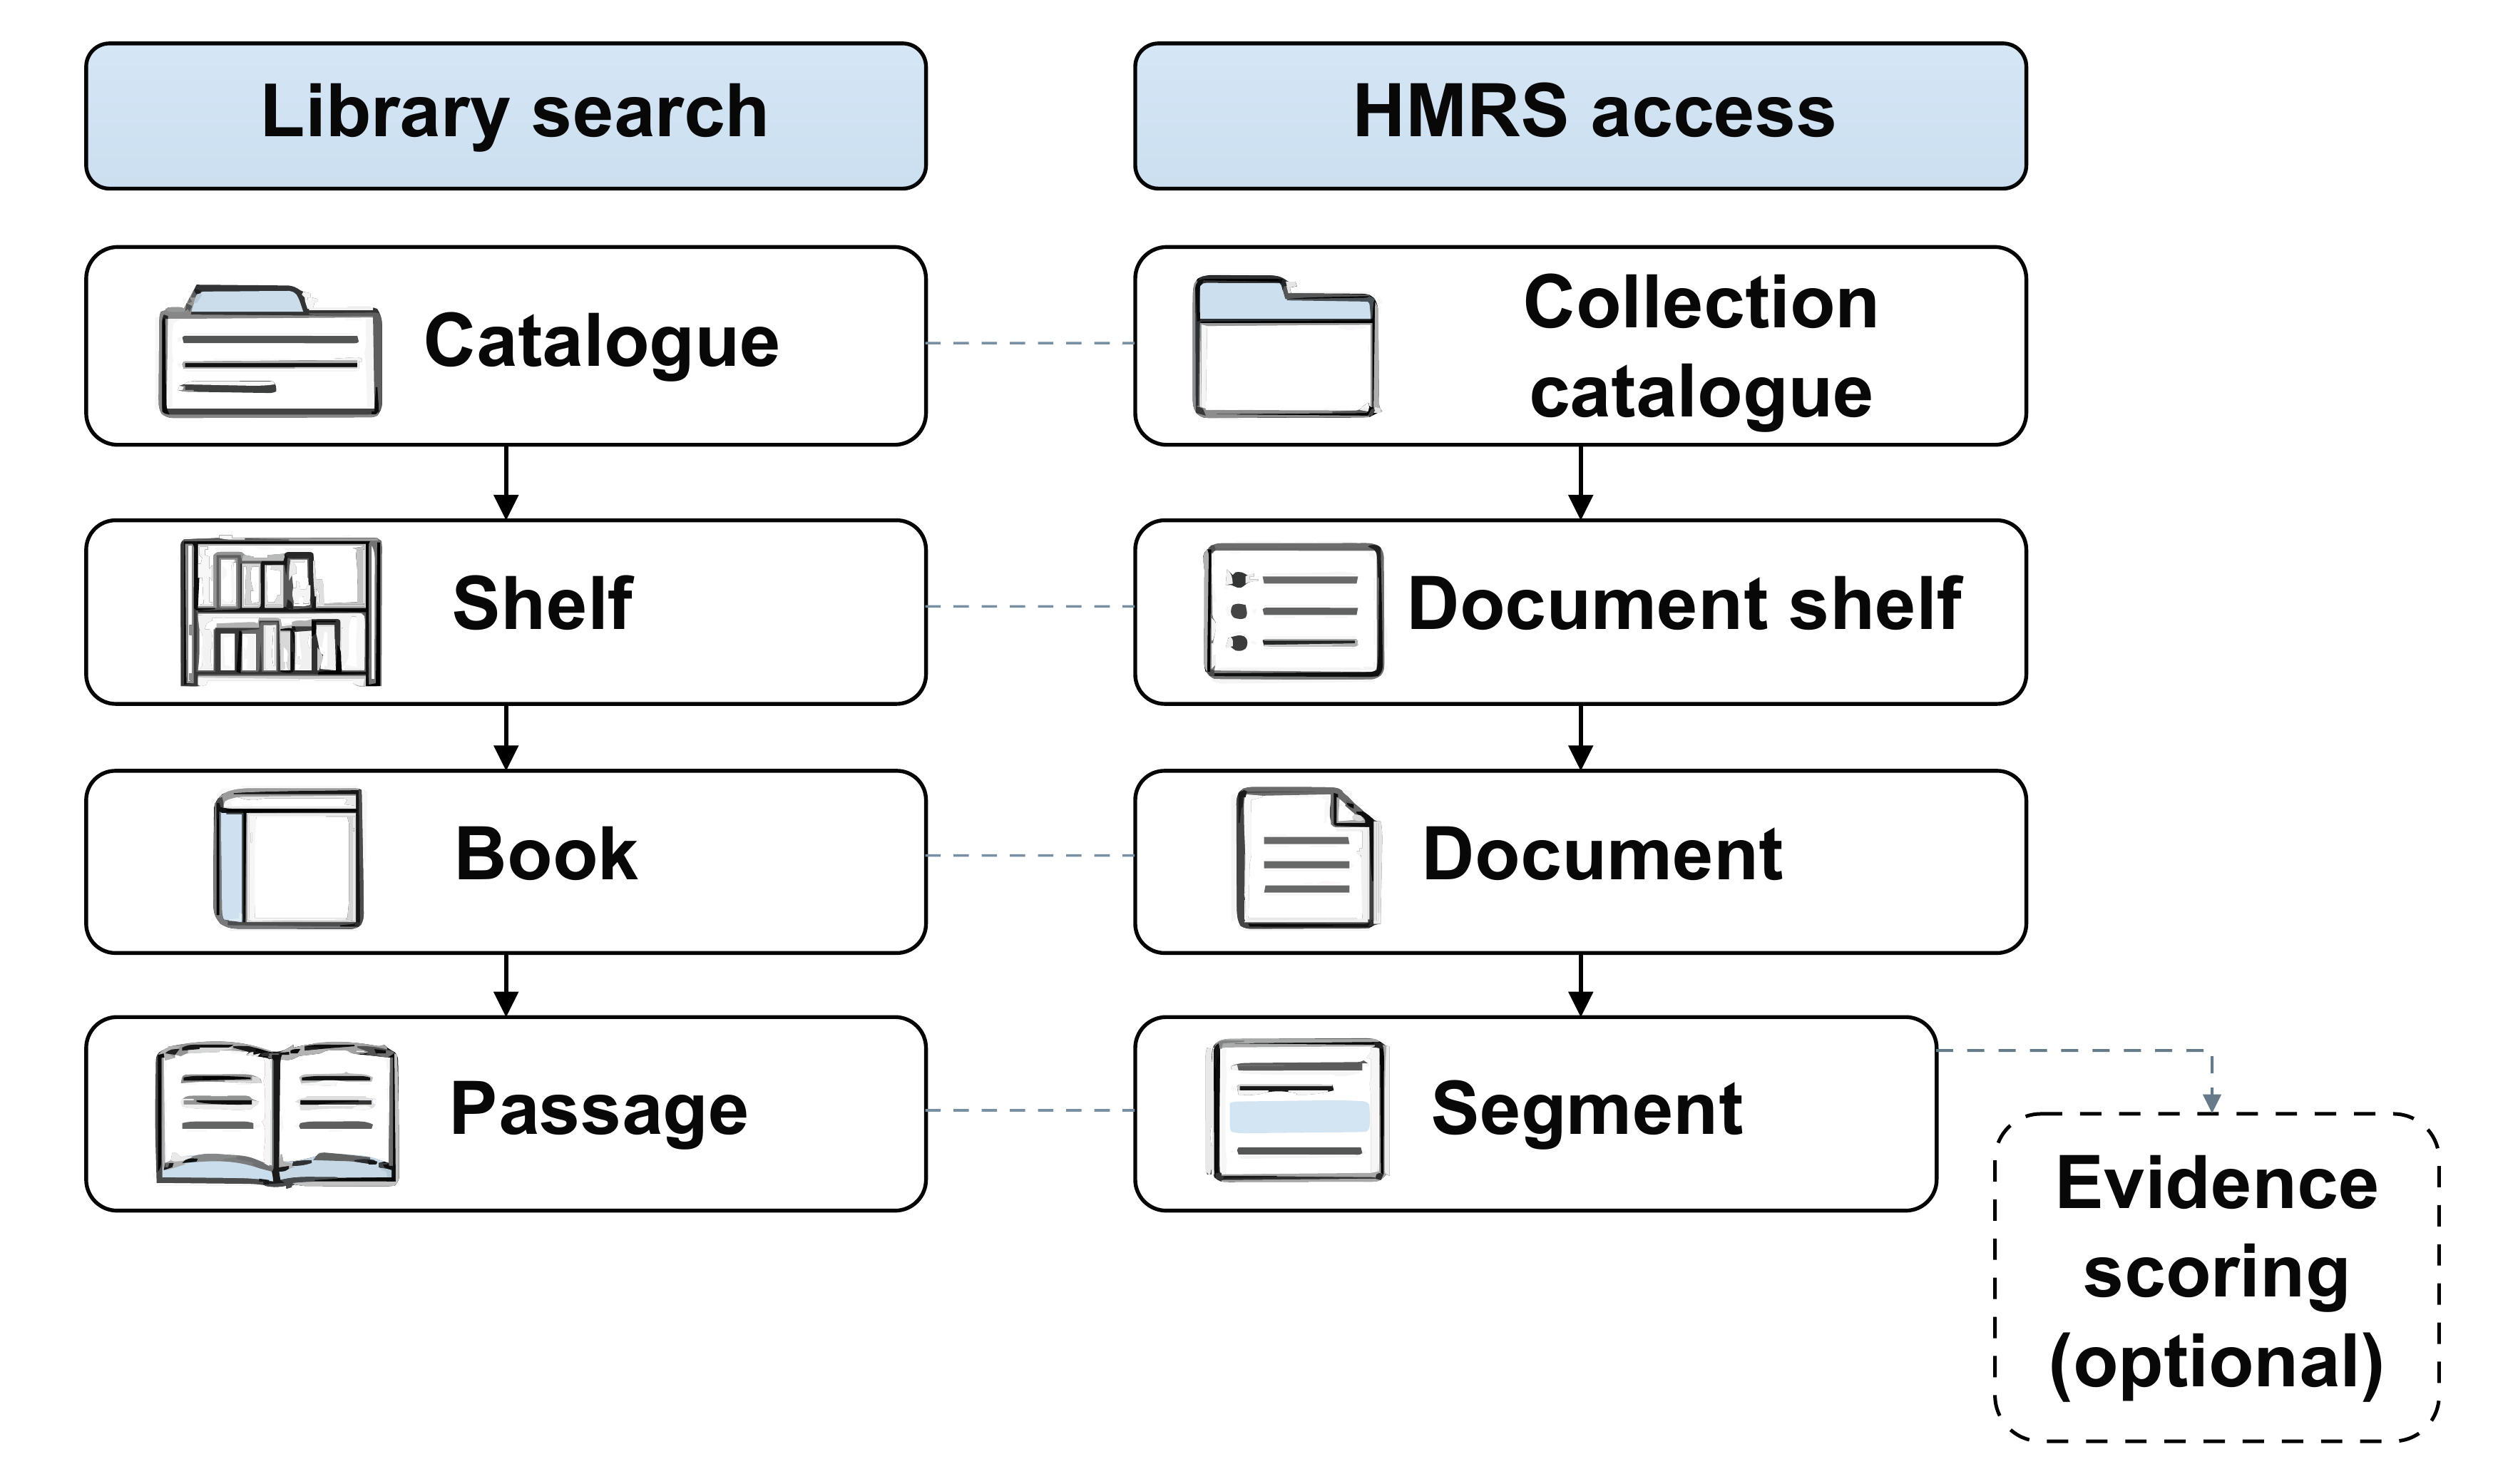
\includegraphics[width=\columnwidth]{figs/fig_library_analogy_vector.png}
\caption{Library analogy for a catalogue-first HMRS access path. The library catalogue, shelf, book and passage correspond to the collection catalogue, document listing, document body and segment. Evidence scoring is optional; pinned search may bypass the catalogue and shelf.}

\end{figure}

\setcounter{dbltopnumber}{1}
\begin{figure}
\centering
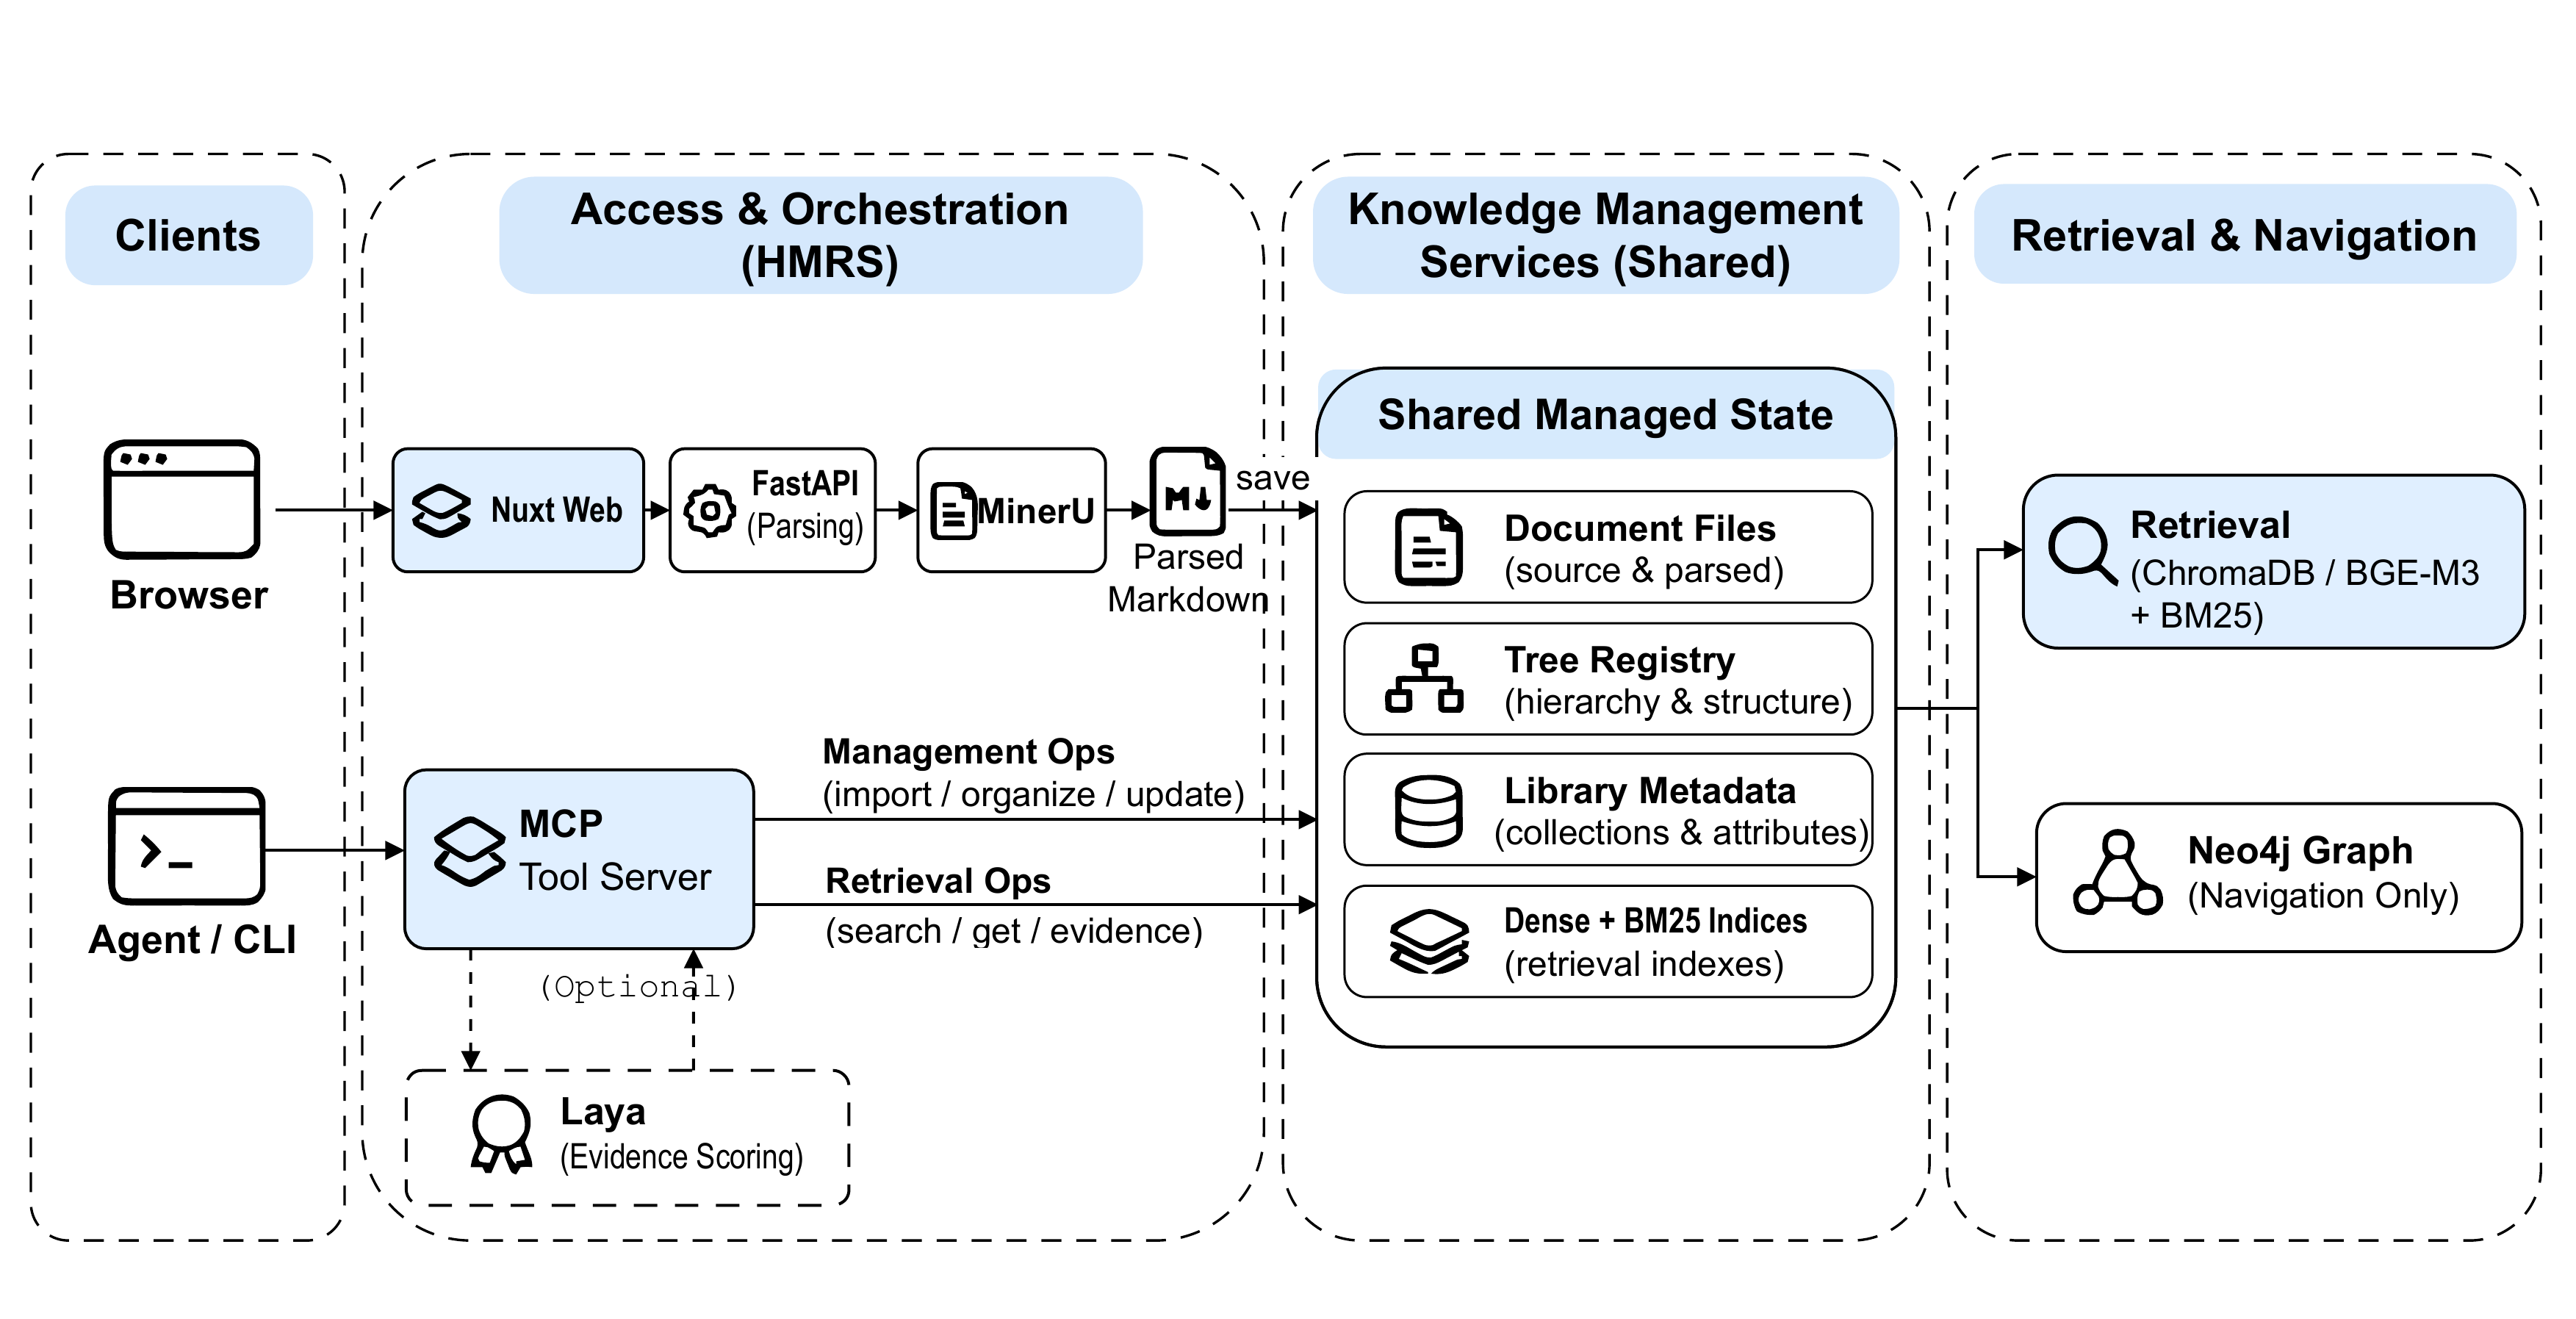
\includegraphics[width=\textwidth]{figs/fig_service_architecture_vector.png}
\caption{HMRS service architecture. The browser and agent/CLI access the web and MCP interfaces. Parsing, management and retrieval operate on shared document files, the tree registry, library metadata and search indices. Laya scoring is optional, and the Neo4j graph supports navigation.}

\end{figure}

Figure~3 summarises an illustrative workflow from document
acquisition and organisation to retrieval and evidence inspection. Parsing is
used when needed; quality review and content-based collection assignment are
agent-workflow procedures, and indexing depends on the entry point. A question
can select documents through catalogue and shelf navigation or through pinned
vector or two-stage search. Laya scoring is optional; incomplete execution is
distinct from a completed review that finds no support. The workflow does not
imply that every step is enforced by the API. The management path covers
acquisition (Section~4), content-informed organisation
and lifecycle checks (Section~5), and the tool and
runtime layer (Section~7). The chat endpoint defines
pinned-search and all-library librarian policies. Hybrid is a composed retrieval
configuration, not a third built-in server policy; it combines vector and
catalogue calls under an explicit directive. The document graph supports
navigation, not evidence. Experience retrieval and the persona-distillation
workflows reuse knowledge-base infrastructure but follow their own retrieval
and filtering paths; neither is described here as invoking Laya, and neither
was evaluated at scale.

The platform exposes five management domains: acquisition, organisation,
lifecycle, query and operational experience. Some controls are enforced by
API/MCP operations; semantic and quality checks are agent-workflow procedures,
and campaign audits test selected outcomes. Table~2
distinguishes these layers and maps each domain to the evidence that exercises
it.

\begin{table}
\centering
\small
\setlength{\tabcolsep}{4pt}
\caption{Management functions, the enforcement or workflow check associated
with each, and the evaluation that exercises it. The table separates API/MCP
controls from agent procedures and campaign audits; semantic choices such as
which collection owns a document remain workflow decisions and are measured,
not enforced.}

\begin{tabular}{@{}p{4cm}p{4cm}p{4cm}p{4cm}@{}}
\toprule
Group & Operations & Platform or workflow check & Evidence\\
\midrule
Acquisition & submit, parse (MinerU), quality review, duplicate review, structural split, store, index & parse-task state; workflow quality checks; entry-point-specific deduplication and indexing; post-index probe & E1--E2, S9\\
Organisation & create library or sub-library, content-informed placement, descriptions and tags, duplicate review & API validates identifiers and required fields; workflow checks descriptions and tags; audit compares files, tree and library metadata & E1--E2\\
Lifecycle & move, rename, delete, force re-index, graph build & operation-specific API updates; reconciliation audit detects selected stale or inconsistent state & E2\\
Query & tier selection, vector, keyword, catalogue and two-stage search, gate invocation & endpoint enforces tool allow/deny lists, timeouts and turn limits; invoked gate returns survivor provenance & E3, E5--E9\\
Experience & extract, approve, tier, search & experience tools apply their own retrieval, verification and credibility filters & E4\\
\bottomrule
\end{tabular}
\end{table}

\begin{figure}
\centering
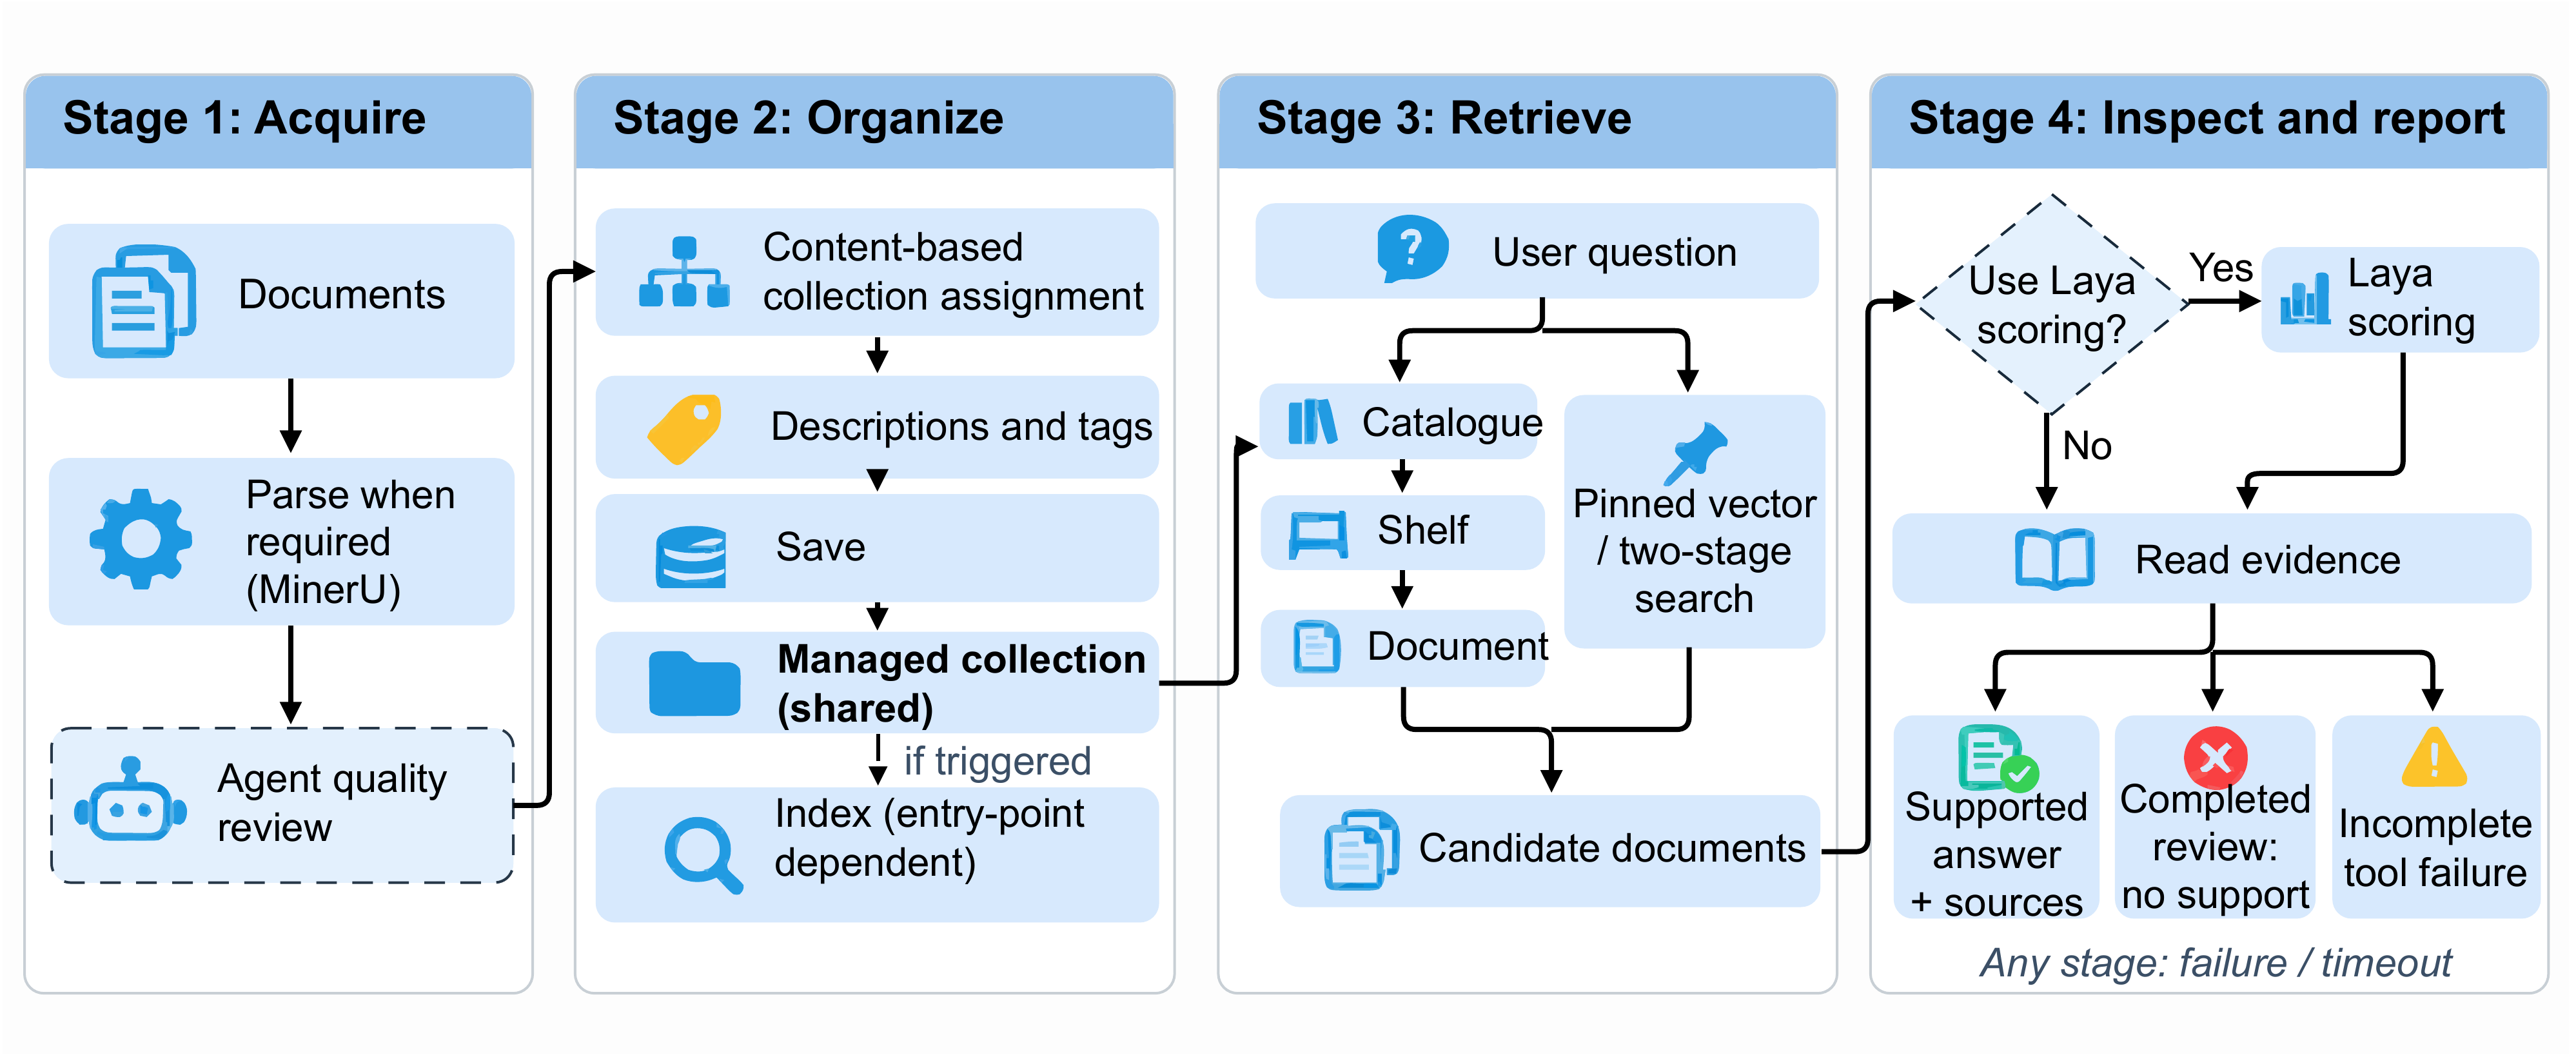
\includegraphics[width=\textwidth]{figs/fig_workflow_vector.png}
\caption{Illustrative HMRS workflow from document acquisition to evidence-based reporting. Documents are parsed when needed, organised into collections and indexed according to the entry point. A question can use catalogue navigation or pinned search; optional Laya scoring precedes evidence inspection. A completed review without support is distinct from an incomplete search or tool failure, which may occur at any stage.}

\end{figure}

\subsection{Data model and object lifecycle}



Documents are Markdown with extracted images. Library state is described by
the document files, the \texttt{.tree-fs.json} registry and each
\texttt{.knowledge-base.yml}. The ingest workflow tracks raw, parsed, stored
and indexed states and can mark completion after its configured retrieval
probe. Indexing is a separate transition: some save paths start vector/BM25
indexing asynchronously, while the web parsed-file save path does not.
Reconciliation detects selected stale-index conditions or disagreement among
the three sources; it is not a cross-store transaction. Because the three
sources are written by different management operations, the collection has no
single authoritative record of its own state, and the reconciliation audit
exists to make disagreement observable rather than to prevent it.


\section{Acquisition and automatic classification: from parsed document to
owned collection}


Acquisition determines what later retrieval can support, and it is where a
document is assigned to the collection that owns it. HMRS submits PDFs,
Office files and scans to MinerU through an asynchronous parsing service
[29]; parse tasks return identifiers that callers can poll, while
workflow quality review examines the resulting text for parsing defects.

The intended ingest workflow includes submission, parsing,
agent-mediated quality review, duplicate review, optional splitting, collection
assignment, storage, indexing and a retrieval probe. These dependencies matter to
the system claim: parsing produces the content used for placement; placement
controls the collections visible to later access; indexing makes the stored
parts searchable; and the probe checks that the claimed transition is visible
through the retrieval interface. Depending on the entry point, artefacts may
include a parse task identifier, a quality report, a content fingerprint, a
split manifest, a storage record, a placement decision and a probe result. The
workflow treats a content-derived retrieval probe as evidence of retrievability;
an HTTP success from a save call alone does not establish that property. The
platform accepts scanned pages, Office files and plain text, but quality review,
classification and completion checks are not all enforced by the parse API.

\subsection{Quality gates and ingest lifecycle}

Duplicate handling has two paths rather than a universal admission gate. The
upload service rejects an exact same-parent duplicate by content hash, while
the separate near-duplicate tool reports similar candidates for review at a
configured threshold; it does not delete them automatically. In the ingest
workflow, an agent reviews parsed text for OCR noise, binary residue, bodyless
headings, whitespace collapse and language mismatch. Save and indexing behaviour
depends on the entry point: the web parsed-file save route stores content
without starting indexing, while the MCP parsed-document save operation can
start vector/BM25 indexing asynchronously. The ingestion agent classifies the document into a library whose scope matches
the parsed content's subject, not its filename, and the classification is
recorded so that the owning collection can be compared with the catalogue
afterwards.

When requested and above the configured context ceiling (30,000 characters in
the arXiv campaign; 60,000 in later configurations), documents are split at
recognised structural markers. The splitter targets 0.85 utilisation as a
soft target and detects units such as headings, Markdown tables, lists, block
quotes and fenced code. It does not guarantee preservation of equation
boundaries. Descriptions and tags are derived from the body and checked by the
ingest workflow; mismatches call for metadata correction, not document
rewriting.
Vector/BM25 indexing and graph construction are distinct operations.
Post-index verification checks selected properties such as a non-empty vector
collection and expected chunk identifiers; reconciliation can detect stale
index state, but is not a transaction across storage and index services.

\subsection{Acquisition evidence and accounting limits}

The 100-paper campaign produced 322 stored parts in five libraries, so the
collection level was populated across five distinct owning collections rather
than a single corpus.
Its reconciliation is incomplete: the state file records 91 submitted names;
at the 2026-10-13 evaluation snapshot 79 papers were retrievable and 21 were
not, and
the surviving artefacts do not enumerate attempts and failures per paper, so
the missing 21 cannot be attributed to parsing alone. Formula-dense scans and
a recovered batch-process crash were observed; neither establishes the cause
for every missing paper.

A separate cross-lingual test processed 400 Wikipedia pages per language.
Ingestion success was 1.0 in both rounds. Automatic membership accuracy was
0.875 for English and 1.0 for Chinese and Japanese; this metric measures
whether content-based classification placed a document in the correct
collection independently of its filename. Section~8.2 reports the
per-language storage and self-retrieval results. These measurements
characterise ingestion, classification and storage, not answer quality.


\section{Collection and document management: organisation, classification and
lifecycle}


Organisation determines which collections exist, which tier can see a
document, and whether the stored state remains trustworthy. HMRS places
documents by content rather than filename; split parts inherit the source
assignment, and the catalogue exposes library and document descriptions
before full bodies are read. This section covers the collection and document
levels of Table~1; the segment level is treated in
Section~6.

\subsection{Classification, metadata, tags and duplicate review}





Integrity checks compare three sources: the document files on disk, the
\texttt{.tree-fs.json} tree and each library's \texttt{.knowledge-base.yml}.
The comparison covers document existence, path and index metadata. Tags derive
from content and are checked against it.
Duplicate detection reports candidate pairs for review; deletion is not
automatic because adjacent parts may be similar while containing distinct
source sections.

The layer's operations are library and sub-library creation, classification,
description and tag edits, move, rename, delete, duplicate review and forced
re-index. Together they implement the management loop that turns parsed content
into a maintained collection: placement records ownership, descriptions expose
scope, lifecycle operations change ownership or content, and reconciliation
checks whether the representations still agree. Each operation updates the
state relevant to it; for example, a move changes the document path and
registry entries, while re-indexing updates search indices. The audit compares
the files and registries where applicable. The catalogue lists libraries, their
descriptions, sub-library containers and document descriptions, which lets a
reader or an agent decide where to look before opening a body. Classification
involves a semantic choice: the ingest agent
selects the library from the parsed content, and the platform checks the
consequences rather than the choice. The same asymmetry holds at query time: the workflow selects a collection,
whereas operations to open and index documents, and optionally score their
segments, are provided by the server.

Sub-libraries are tree nodes with their own descriptions and indices. For a
parent scope, the vector service resolves the parent and its descendants to the
collections available to that query; the two-stage service likewise resolves
descendant identifiers during its lexical stage. This is a scope-resolution
policy, not a claim that child vectors are stored in the parent's collection.
The measured campaigns used explicit per-library scopes for the flat union and
did not treat parent traversal as an independently benchmarked retrieval
condition. Index availability and route-specific failures therefore still
require a post-search probe.

\subsection{Lifecycle operations, graph and operational knowledge}




A historical rename trial left stale vector chunks until forced re-indexing.
The current rename path starts index synchronisation asynchronously, with
failures logged as non-fatal; checking the resulting index remains necessary
because successful metadata updates alone do not establish index consistency. The document graph supports navigation and candidate
expansion, not evidence. Operational lessons are stored as retrievable
documents with credibility tiers, but the available measurements are case
examples rather than a scale evaluation of distillation, approval or
credibility decay.

\subsection{Organisation contract}



The evaluation checks three-source consistency, content-derived descriptions,
regression probes and lifecycle outcomes (Section~8.3). Reconciliation
can expose selected stale or inconsistent states; it does not detect or prevent
every failure by construction. Merge and split remain outside the controlled test
scope, so performance claims must be read within the corpus sizes reported in
the Evaluation section.


\section{The tiered access path: from collection to admitted segment}



The access path reads the collections, catalogue and indices maintained by
acquisition and organisation. It is the query-side counterpart of the
management levels: the catalogue tier chooses a collection, the shelf tier
chooses documents within it, the document tier opens a body, and the segment
tier can score its parts. Two built-in chat policies and an experimental
composition use different affordances of that path, and a calling workflow may
invoke the separate server-side Laya evidence gate. The tool fetches referenced document text, segments it and applies a
local, query-conditioned verdict. Its model-card field (\texttt{noul}) is a
typed 0--1 score; this study reports no probability-calibration experiment and
does not interpret the score as a calibrated probability. Segments meeting the
configured threshold (0.5 by default) are returned as survivors with
provenance. A scored segment below the threshold is not admitted, while tool
or fetch failures are reported separately; a partially completed call may
still return successfully scored survivors. The answer workflow reserves a
scoped not-found report for a completed search with no supporting evidence,
not for an execution failure.

An access workflow can combine the following operations. Their order and
inclusion depend on the entry point and the question; the list is not a
server-enforced sequence for every query.
\begin{enumerate}
\item \emph{Rewrite.} The agent forms retrieval queries from the question.
\item \emph{Gather.} A pinned search calls two-stage or vector search; a
catalogue-first search selects collections and document descriptions. A
composed workflow can combine candidates from more than one source.
\item \emph{Merge and cap.} Where multiple sources are combined, the workflow
can deduplicate and limit the candidate set. Specific limits are properties of
the evaluated configuration, not universal platform guarantees.
\item \emph{Judge.} When invoked, the gate fetches candidate documents, scores
segments and returns survivors with provenance; fetch and tool failures are
reported separately from low scores.
\item \emph{Read and answer.} The agent examines the evidence pack and may read
a surviving document to check a specific claim before synthesising an answer.
\end{enumerate}

Figure~4 summarises this workflow and its terminal
conditions; Algorithm~1 expresses the same decision sequence
in pseudocode. Both are workflow abstractions: individual entry points may
omit or combine candidate-gathering steps.

\begin{figure}
\centering
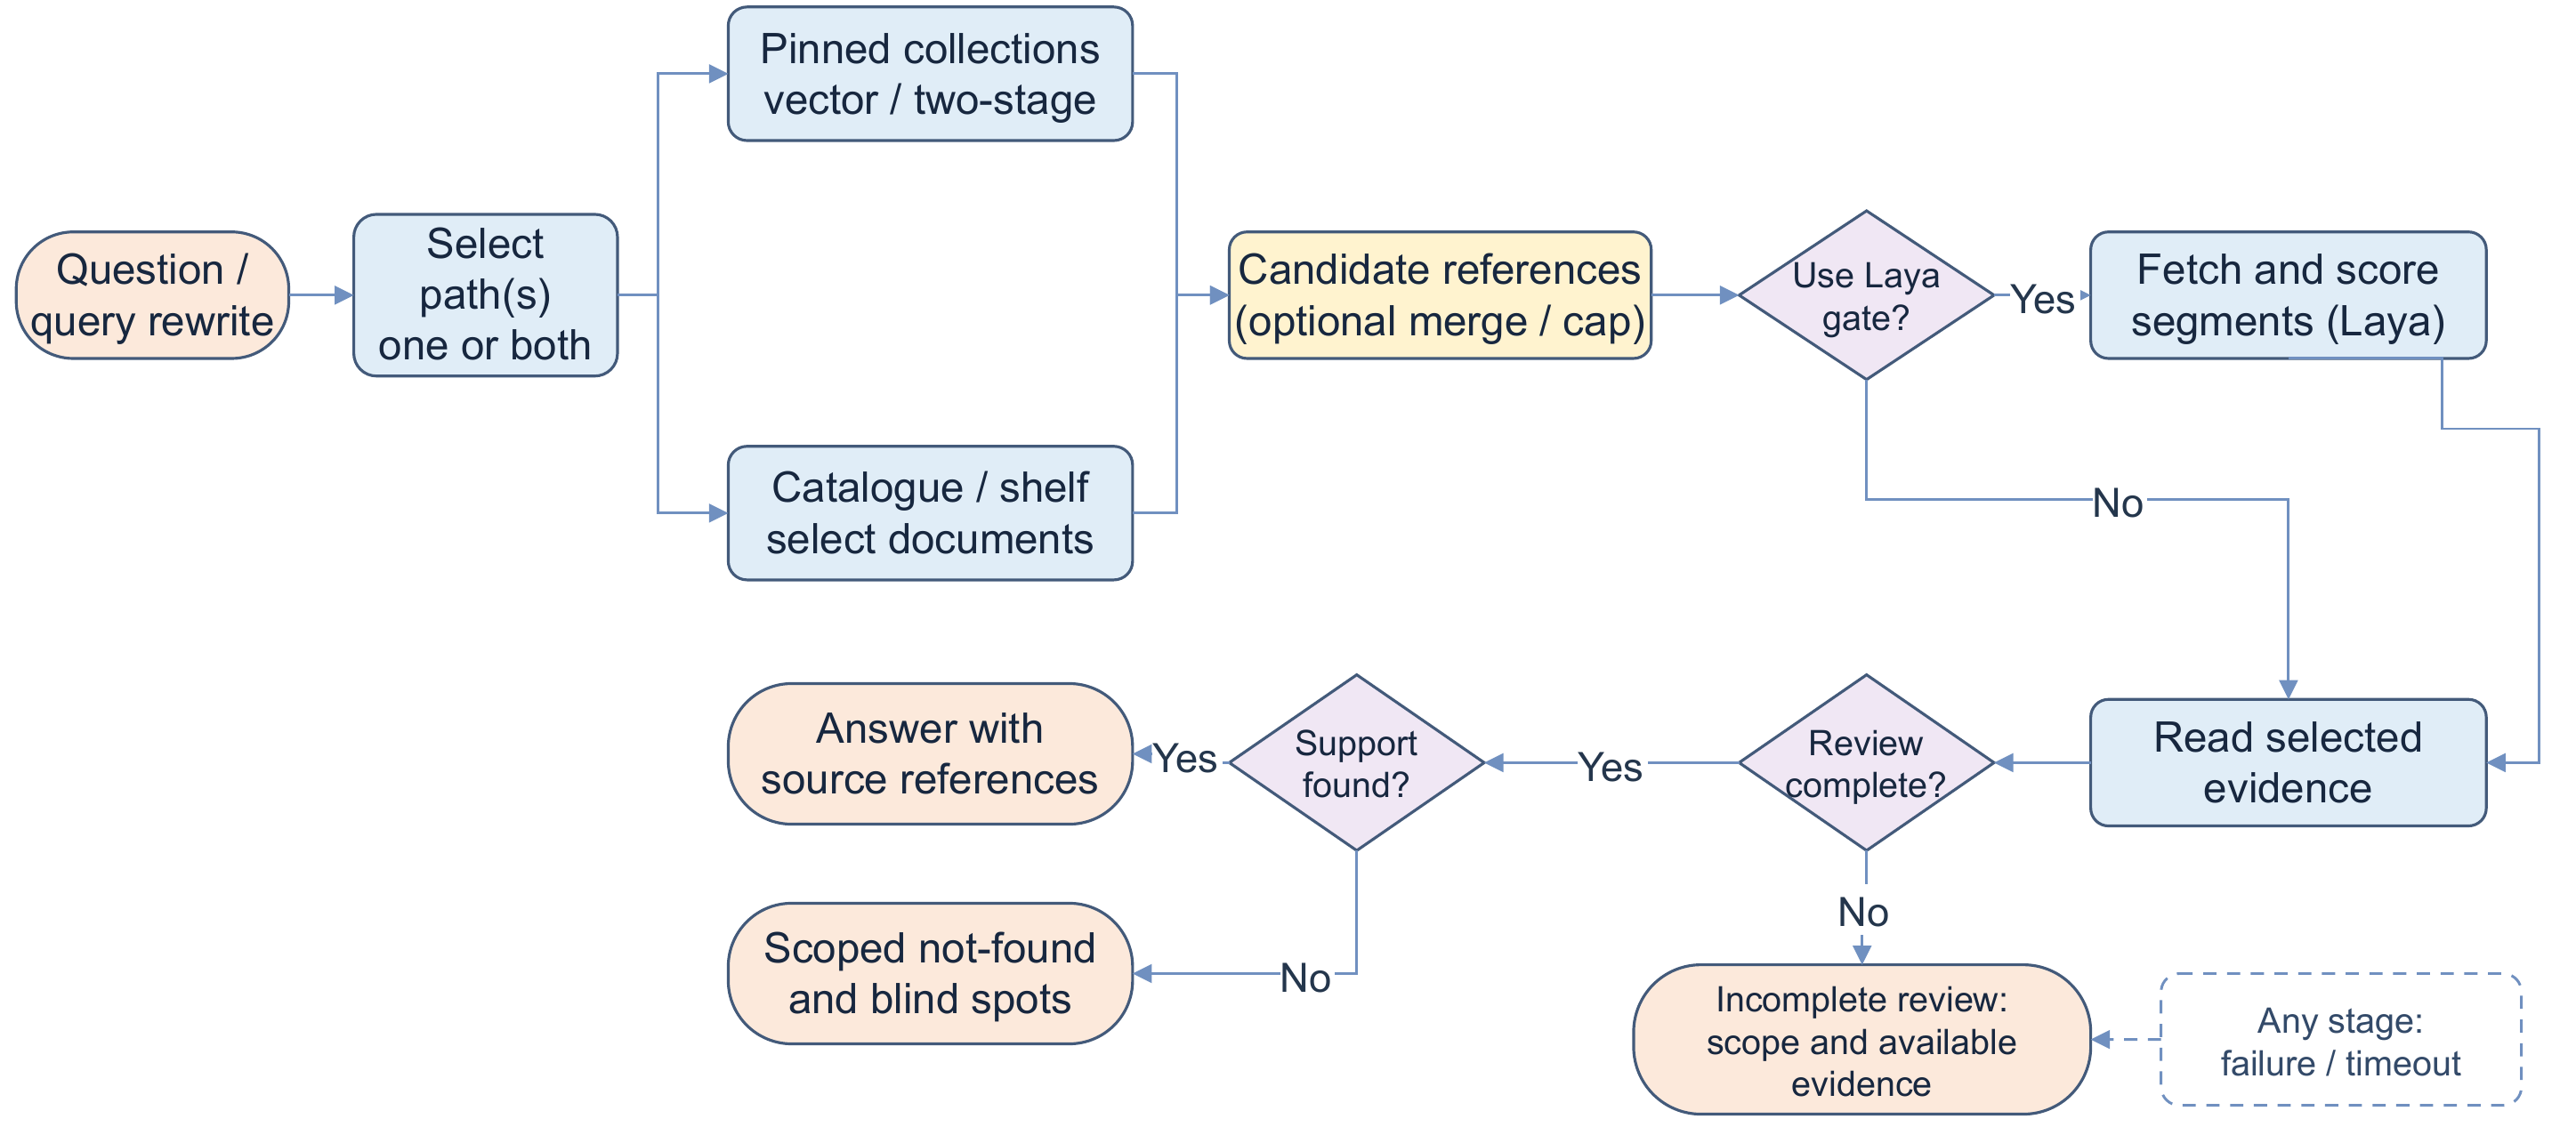
\includegraphics[width=\textwidth]{figs/fig_tiered_drawio_20261116.png}
\caption{Tiered access workflow. Candidate references can be gathered from
pinned collections, catalogue navigation or a combination. The optional Laya
gate fetches and scores segments. An incomplete operation at any stage reports its scope and any
available evidence; a scoped not-found is reserved for a completed review
without support. The workflow describes intended agent behaviour, not a
server-enforced sequence.}

\end{figure}

\begin{algorithm}[t]
\caption{Tiered access with optional evidence gate}

\begin{algorithmic}[1]
\Require question $q$; catalogue $\mathcal{C}$; threshold $\tau$; gate flag $g$
\State $D \gets \textsc{GatherCandidates}(q,\mathcal{C})$ \Comment{pinned or catalogue-first}
\If{$g$}
  \State $S \gets \textsc{LayaJudge}(D,q,\tau)$ \Comment{fetch, score and return survivors}
\Else
  \State $S \gets \textsc{ReadSelected}(D)$
\EndIf
\If{execution incomplete}
  \State \Return incomplete status, searched scope, and available evidence
\ElsIf{completed review finds no support}
  \State \Return scoped not-found (searched scope, blind spots)
\Else
  \State \Return agent-synthesised answer with source references
\EndIf
\end{algorithmic}
\end{algorithm}
Exhausting a policy's call budget is intended to produce a scope and blind-spot
report. The endpoint enforces timeouts and turn limits; the per-policy budgets
are workflow instructions, not server quotas.

\subsection{Tier policies and the evidence gate}





The current chat instructions provide two retrieval modes. In pinned mode,
the agent rewrites the question and calls the two-stage search (preferred) or
vector search within the selected collections; it can send candidate references
to Laya in sequential batches and optionally open a survivor for a specific
quote. In all-library mode, the instruction walks the catalogue and selected
shelves, selects document references from descriptions and sends these to Laya
before reading survivors. These are agent instructions, so actual tool use is
reported from traces rather than assumed from the instruction. Endpoint-level
timeouts and turn limits bound execution; retrieval sequences and batch sizes
are workflow instructions rather than separate server-enforced per-lane quotas.

The experiments also use fixed retrieval configurations. In particular, the
historical hybrid wrapper whose logged pools are analysed in
Section~8.9 is no longer a
registered tool. Another controlled candidate-pool experiment uses per-library
vector top-30 at cosine threshold 0.35 together with catalogue candidates,
followed by fusion and a twelve-candidate cap. These values identify that
experiment, not the current chat default. A composed hybrid directive may call
vector and catalogue tools in an agent workflow. Table~3
summarises the current modes and the evaluated composition.

The gate is the local Laya evidence classifier [89], exposed as
\path{kb_laya_judge}. In reference mode, the server fetches candidate
documents, scores their segments against the query and returns surviving
segments with provenance and a bounded evidence pack. This is a threshold-based
admission operation; it does not itself fuse candidate sources or impose the
workflow's top-$k$ reading window. Those decisions belong to the calling search
configuration or agent workflow. To construct the evidence pack, the tool
orders surviving segments by source and position, deduplicates them and applies
the character limit. A passing verdict
is not proof of truth or entailment; the verifier remains subject to calibration
and transport limitations.

\begin{table}
\centering
\small
\setlength{\tabcolsep}{5pt}
\caption{Access policies over the tiered path. Modes differ in how candidate collections and documents are selected.
The hybrid row describes an experimental composition.}

\begin{tabular}{@{}p{4cm}p{4cm}p{4cm}p{4cm}p{4cm}@{}}
\toprule
Policy & Tiers traversed & Retrieval affordance & Budget type & Intended terminal report\\
\midrule
Search & pinned collections, segment & Two-stage or vector search & Endpoint turn limit & Answer or report not-found\\
Librarian & catalogue, shelf, document, segment & Catalogue navigation and optional judging & Workflow instructions & Scope and blind spots\\
Hybrid & catalogue and segment & Composed vector and catalogue calls & Configuration-specific candidate cap & Candidates or judged survivors\\
\bottomrule
\end{tabular}
\end{table}

The two-stage tool builds a candidate pool with lexical search and optional
graph expansion, then applies dense ranking. It does not call the
evidence gate; a ranked chunk does not by itself establish evidential support,
and a similarity threshold is not an abstention mechanism. The 13 October catalogue
incident showed that oversized tool returns can conceal documents before
reasoning begins. The tested repair adds a server-side character budget,
grouped views and pagination; its behaviour is reported in the Evaluation
section.

\subsection{Honest abstention}
A candidate list may contain high-similarity but unsupported documents. The
answer workflow instructs the agent to report not-found when its completed
evidence review finds no support, including the searched scope and known blind
spots, rather than falling back to parametric knowledge. This behaviour was
observed in the reported trials; it is not a server-side semantic-classifier
guarantee. Timeouts, unavailable tools and incomplete searches are execution
failures, not evidence of semantic absence (Section~8).


\section{Agent interface and implementation}



\subsection{MCP tools and lane policy}


The platform exposes MCP tools across management and retrieval categories. They
fall into the management groups of Table~2: parsing and
quality review for admission, library and sub-library creation, placement,
description and tag editing for organisation, move, rename, delete and forced
re-index for lifecycle, catalogue, vector, keyword and two-stage search for the
access path, the Laya evidence gate for segment admission, the document graph
for navigation, and operational-experience tools. These tools support a
closed operational loop: a write changes managed state, a read or probe checks
the resulting state, and a re-index or reconciliation operation makes stale
state visible or repairable. Persona-distillation workflows are outside the
scope of this evaluation and use their own retrieval and synthesis path.
Access policies receive read-oriented tool sets; administrative writes remain
separate, and long-running parse, re-index and graph operations return
pollable task identifiers. Figure~S1 summarises the software design: a tool
layer over management services that share one auditable state, with the
evidence gate as an optional segment-level call.



The chat endpoint adapts multiple agent harnesses to the lane interface. The
server selects a harness and permission mode, enforces configured tool
allow/deny lists, applies endpoint timeouts and turn limits, and may register an
asynchronous task. Lane-specific retrieval sequences and call budgets are
workflow instructions; the endpoint does not enforce a separate per-lane call
quota.

\subsection{Runtime and deployment}


The backend uses Python 3.12 and FastAPI. ChromaDB stores cosine-space HNSW
collections with normalised BGE-M3 embeddings (1024 dimensions)
[48,90,91]; Neo4j stores the document graph [92];
BM25 supports lexical search [7]; MinerU provides parsing and OCR
[29]. The Laya verifier runs locally as a serialised worker.

The evaluation environment is one self-hosted Windows workstation with an
RTX 5060 (8 GB) used for embeddings and judging. Local execution reduces
external service dependencies but does not establish privacy, access-control or
multi-host deployment guarantees. A stack-ensure script checks the API, web
front end and MCP endpoints and can restart missing services before an
end-to-end retrieval probe. Three recent acceptance trials reported recovery
from a stopped stack without manual intervention. This is an operational
observation, not a guarantee of availability in every deployment.

The implementation and scripts are available
at \url{https://github.com/kingdol666/rag-knowledge}; experimental corpora
remain subject to their data-use constraints.


%% n8a_eval.tex -- evaluation, first part: roadmap, design/measures, E1
%% (acquisition), E2 (organisation/lifecycle) and E3 (route-card audit).
%% Numbering follows the 2026-11-13 map (E3 = route audit, E4 = experience);
%% labels are historical and remain unique: sec:eval, sec:eval-setup, sec:e1,
%% sec:e2, sec:routing-audit, fig:routing, tab:eval-design.
\section{Evaluation}

We evaluate HMRS as a knowledge-management system with an access path, not as
an isolated ranker. Three evidence families are kept separate and are never
pooled into a system-level accuracy: management (E1--E2 and E4), access (E3
and E5) and answer/deployment (E6--E7), with E8 diagnosing verifier
placement and E9 bounding stability, concurrency, gate and scope behaviour.
E3 tests scripted collection choice and E5 measures retrieved text on the
same question set; E6 uses separate questions to inspect answers and traces.
In research-question terms, E1, E2 and E4 answer RQ1; E3 answers the
collection-selection part of RQ2; E5 answers RQ3; E8 answers RQ4; E6 and E7
answer RQ5; E9 bounds all five questions. Table~S17 records the design and
provenance of each campaign; Tables~S9--S10 group the management
observations and retrieval designs with their limits.

\subsection{Experimental design and measures}


\textbf{Corpora and questions.} Five data packages are used, each with its own
unit. The industrial demonstration corpus contains 42 documents in five
libraries, including twenty near-duplicate telemetry reports, and 16
developer-authored questions with gold document fragments; Q16 shares a token
with its gold filename. The arXiv campaign submitted 100 papers across about
25 domains and produced 322 stored parts in five libraries at the 2026-10-13
snapshot; its ten gold questions are keyed by arXiv identifiers. A later
re-check enumerated 328 parts in the same five libraries and audited their
descriptions; it is a separate state, not a matched rerun. The cross-lingual
ingestion corpus has 400 Wikipedia pages per language (English, Chinese and
Japanese) and 40 extractive queries per language; its index self-check is not
a task-level retrieval benchmark. A separate routing corpus has 138 documents
in 879 parts across ten domains, 72 in-domain questions and four
out-of-domain probes per arm; two cross-placeholder probes are excluded. The
same 72 questions were rerun as a same-question follow-up whose corpus grew
to 906 parts; it is not an independent sample. The packaged trace tables
retain 76 question IDs per complete arm; four R1--R4
cross-placeholder/out-of-domain probes remain in the CSV. They are excluded
from the 72-question in-domain containment and paired tests, and are not
pooled into an abstention-success rate. Questions and gold annotations were
developer-authored, not sampled user queries.

\textbf{Measures and controls.} Document-level Hit@5, Recall@5 and MRR@5
measure the returned top five, with MRR zero if no gold appears in that
window [93]. Scripted route accuracy checks the
labelled collection, whereas annotated target-string containment checks
whether the target substring occurs anywhere in the returned evidence pack;
a sibling-document occurrence may count, so this is not gold-document
retrieval, entailment or semantic answer correctness. Automated RAG evaluation frameworks [94] assess the semantic quality of generated answers,
while cumulated-gain measures [96] evaluate
graded relevance of ranked results; neither is used to score semantic answer
quality here. The answer grids check whether the gold identifier appears in
the answer or trace, whether at least $\lceil3n/5\rceil$ annotated terms are
present (strict) or an accepted alias (alias-aware), and whether a
document-style citation marker is present. A marker does not establish source
resolution or entailment. Wilson intervals are conditional on the questions
and run. Exact McNemar tests are exploratory, two-sided and unadjusted; no
familywise inference is intended across the listed contrasts. Agent arms use
one model and one run per condition; retries after transport failures are
not independent repeats. The answer-layer campaigns used the platform chat
API (Claude Code engine); the four-question harness case compared Claude
Code with oh-my-pi pinned to the ustc/deepseek-flash model (November 2026).
Two corpus-integrity defects were
repaired before measurement, so their natural failure rate is unknown.
Table~S17 records these boundaries; Tables~S9--S10 map
management functions and campaigns to their checks.

\subsection{E1: Acquisition and parsing}

The 100-paper campaign recorded 322 parts in five libraries. At the October
snapshot 91 paper names appeared in the ingest state and 79 papers were
retrievable: twelve recorded and nine unrecorded papers were not retrievable,
and the records do not establish per-paper parse status or the stage causing
each failure. A later re-check enumerated 328 parts in the same five
libraries and found a content-derived description for every part (328/328,
at least 60 characters, with no placeholder names), a metadata result
separate from retrieval accuracy. The same re-check ran a filename-stem
short-query identifier probe: a query built from each PDF filename stem was
searched in result names for the arXiv ID. The ID appeared for all 100
records after forced reindexing, explicit indexing and a probe-tool
correction. This is an identifier-visibility diagnostic, not scoped title
retrieval: 72 records did not specify a library and 45 returned a chunk-copy
name first. It is not a matched before--after comparison with the October
snapshot. A separate ten-question vector check, scoped to the five
libraries, placed the gold document first in all ten questions and invoked
the judge with its real engine in all ten; the retained summary does not
preserve complete judge inputs, so survivor and evidence-pack counts are not
reported as a 10/10 result. The cross-lingual test ingested 400 pages per
language with membership 0.875 for English and 1.0 for Chinese and Japanese;
its post-ingest self-retrieval is an index check, not a task-level
benchmark. A separate 50-paper, 26-domain campaign parsed and verified all
papers, but 41 negative tag flags did not block ingestion and no other
quality-review outcomes were recorded.

\subsection{E2: Organisation, consistency, and management operations}

The consistency checks show that the three-source state is auditable and
repairable, not that every operation is correct. A disposable-library rename
left stale chunks in the vector index: 18 instead of nine, with duplicate
results; forced re-index restored nine. The 322-part campaign passed its
content check on all parts and its three-source checks on a 33-part sample.
A disposable three-level fixture supported parent-to-child moves, listing,
reading and judging. Of 16 lifecycle scenarios, create, move, delete and
forced re-index passed, while task-status reporting and the update check
failed; merge and split were not controlled. Near-duplicate review over the
322-part corpus at a 0.90 threshold reported 35 candidate groups
(0.90--0.975) with zero true duplicates and deleted nothing (Table~S9).
Tag checking passed 165 parts,
while orphan tags and one cross-library registry leak were observed. The
graph supplies navigation rather than evidentiary support: a document move
changed four tag edges (4,675 to 4,679) on a 658-node graph, which is a
navigation record, not evidence. These results motivate reconciliation
without establishing its completeness.

\subsection{E3: Paired route-card audit: the description-layer ablation}

The collection tier is audited as a paired description-layer contrast: route
cards carrying derived descriptions (A0) against nominally name-only cards
(A3), on one fixed question set. A scripted route-card probe returned the
labelled domain for 72/72 in-domain questions in A0 and 37/72 in nominally
name-only A3; 35 routes were correct only in A0
(Figure~5a; exact McNemar $p=5.82\times10^{-11}$).
Evidence-pack containment was 37/72 for A0, 33/72 for A3 and 72/72 for the
mechanical read-all arm (Figure~5b; A0--A3 10:6,
$p=0.4545$; read-all--A0 35:0, $p=5.82\times10^{-11}$). The frozen traces
recorded 31.4 KB and 16.3 s per A0 question, 309 KB and 13.8 s per A0h
question, and 24.3 MB and 253.7 s per read-all question
(Figure~5c); the read-all scan issued 64{,}584 document-read
calls in total, about 897 per question. These are tool-side text and
tool-time observations, not network traffic, model input or end-to-end
latency. Read-all is a mechanical string scan, not an answering agent.

The contrast is a configuration diagnostic, not an independent agent-selection
test. An unlogged A3 fallback could read descriptions; some questions share
titles with route-card descriptions; A3 can search outside the evaluation
scope; and 52 of the 72 questions were automatically expanded, with 47 from
three domains. The difference therefore does not isolate the effect of
descriptions. It does show that the route card and the returned evidence are
separate tiers: A0 finds the collection in every question while A3 does not,
and the evidence pack can still miss the string when the collection is
correct (A0 37/72 containment). The read-all arm bounds what a full scan can
find, at about 78 times the recorded text of A0h; it says nothing about
careful reading or answer quality. The content-layer configurations, in
which the tiered chunk-window arm A0h reaches 51--52/72 containment, are
reported in Section~8.6; the 37/72 figure above is this
audit's own route-card evidence-pack containment.

\begin{figure}
\centering
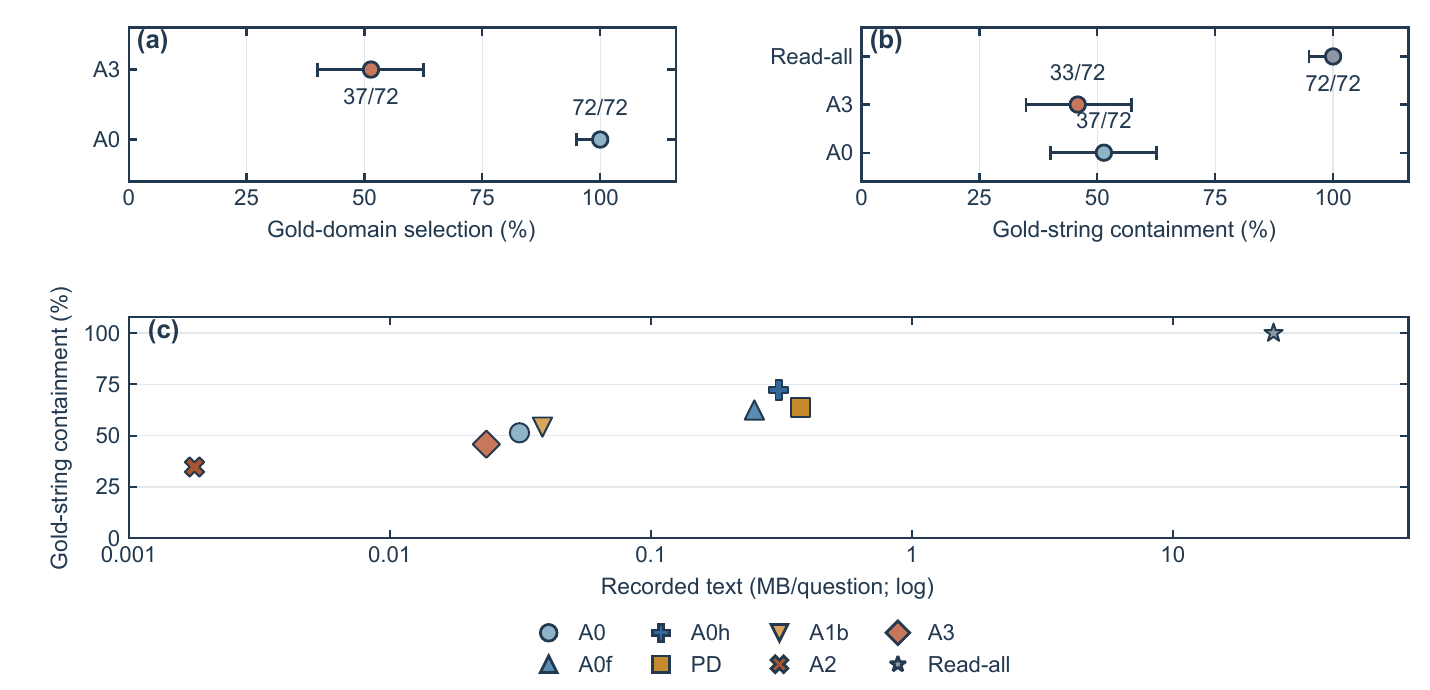
\includegraphics[width=\textwidth]{figs/fig_opt_route.png}
\caption{Route-card diagnostic on 72 in-domain questions. (a) Gold-domain
selection: A0 72/72, A3 37/72; Wilson 95\% intervals; 35 A0-only routes, exact
McNemar $p=5.82\times10^{-11}$. (b) Exact annotated target-string containment in the returned pack: A0 37/72,
A3 33/72, mechanical read-all 72/72; A0--A3 10:6 ($p=0.4545$), read-all--A0
35:0 ($p=5.82\times10^{-11}$). (c) Frozen trace-recorded text per question
(MB, log scale) against containment; A0h 0.309 MB/72.2\%, read-all 24.3
MB/100\%, A0 0.031 MB/51.4\%. In panel (c), the A0f and PD markers are
shifted horizontally by 8 pt solely for visibility; the summary data retain
their unshifted coordinates. Read-all is a mechanical string scan, not an
answering agent; A3 has an unlogged fallback and may search outside the
evaluation scope; tool time excludes answer generation. These are routing,
substring and text-volume diagnostics, not answer quality or an isolated
description effect.}

\end{figure}


%% n8b_eval.tex -- evaluation, middle part: E4 (operational knowledge and
%% automated distillation) and E5 (content-layer configuration comparison).
%% Labels owned here: sec:e3 (E4, historical name), sec:ladder-opt (E5),
%% fig:content. The former fig:ladder / fig:miss-overlap floats and the
%% separate R3 follow-up figure were merged into fig:content on 2026-11-16.
\subsection{E4: Operational knowledge and automated distillation}


The experience store is a functional observation, not an effectiveness
result. It holds operational lessons as retrievable documents---addressed,
indexed and searched as an ordinary document, with a credibility tier
deciding whether a lesson may be shown
(Section~5.2). Three case measurements exist: an
extraction campaign over one small knowledge base produced thirteen
candidate drafts; one end-to-end scenario was sedimented into one experience
(\texttt{exp-d6f4d47ae3d6}) that a later global experience search returned
first, at local similarity 0.711; and the draft-approval path was never
exercised, because the draft pool was empty (\texttt{count}~0) and the read
and approve operations could not run. The heuristic extraction path had run
only in dry-run mode, returning a dump the quality gate would reject. One
scenario and thirteen candidates cannot support an effectiveness claim;
scheduled distillation, review and approval at scale, application feedback
and credibility decay went unexercised.

\subsection{E5: Content-layer configuration comparison}

A0 is the tiered baseline with route-card selection and a 40K reference-mode
judge. A0f retains route-card selection but reads full document windows
inline (up to 250K characters); A0h adds the top-eight vector-chunk windows
to A0f, with a 60K evidence cap. PD removes catalogue navigation and
searches a per-library top-six document union before full-window judging.
A1b is a scoped union of vector results from the ten evaluation libraries,
merged by score and judged in a 40K reference window; A2 uses the same
scoped vector union with concatenated candidate snippets and no judge. A3
uses nominally name-only route cards, while read-all mechanically scans
every stored part for the target string. Route-card retrieval uses
top-30 vector candidates at cosine threshold 0.35 with a 0.30 retry. These
are recorded configuration details, not a single-factor design: A0h, PD and
A1b vary in routing, candidate construction and judging, so their
differences cannot be assigned to navigation alone. Some reference lookups
may use the gold domain, with unknown frequency and impact; A3 may retrieve
outside the evaluation scope.

\textbf{A0h had the highest annotated target-string containment among the
four completed content arms in each execution.} In the frozen aggregate, the
target string occurred somewhere in the returned evidence pack for
A0/A0f/A0h/PD/A1b/A2/A3/read-all in 37/45/52/46/39/25/33/72 of 72 questions
(Figure~7a). A hit can occur in a non-gold sibling document;
this is a lexical evidence-pack proxy, not gold-document retrieval, entailment
or answer correctness. The A0h Wilson 95\% interval is [0.610, 0.812]. The four
content arms (A0, A0f, A0h, PD) were executed three times: the frozen run,
an archived reproduction of it recorded to retain response texts, and a later same-question follow-up on a
corpus grown from 879 to 906 parts (the R3 record). A0h
was the highest configuration and the ordering A0h $>$ PD $>$ A0f $>$ A0
held in all three records (52/46/45/37, then 51/45/44/39 twice). The
reproduction agreed with the frozen records on 71/72 questions for A0f, A0h
and PD and on 68/72 for A0, and the follow-up returned hit/miss records
identical to the reproduction for all four arms. A1b and A2 repeated their
frozen counts exactly in the follow-up, with no per-question flips; frozen
versus follow-up agreement was 94.4\% for A0 and 98.6\% for A0f, A0h and
PD. The follow-up reuses the frozen questions, so these are stability
records, not independent test sets.

In exploratory paired records (two-sided exact McNemar tests, unadjusted; no
familywise inference is intended), A0h led the tiered baseline A0 on
fifteen frozen questions with no reverse ($p=6.1\times10^{-5}$) and on
twelve follow-up questions with no reverse ($p=0.00049$). A0h led the
scoped flat union A1b on thirteen frozen and twelve follow-up questions,
again with no reverse ($p=0.00024$; $p=0.00049$). A0h led PD on seven
questions in both records while PD led on one ($p=0.0703$); this contrast
is not statistically resolved, and PD differs from A0h in more than
navigation. The window expansion is supported separately: A0f led A0 on
eight frozen questions with no reverse ($p=0.0078$) and on five follow-up
questions ($p=0.0625$), and PD led A0 on six follow-up questions with no
reverse ($p=0.031$). A1b and A0 showed no resolved difference in either
record (frozen 2--4, $p=0.69$; follow-up 1--1). Removing the evidence gate
is the clearest isolated cost: A2 contained the string for 25/72 against
37/72 (frozen) and 39/72 (follow-up) for A0, with discordant records of
6--18 ($p=0.0227$) and 5--19 ($p=0.0066$). A2 and A0 also differ in
returned text, so even this comparison does not isolate the gate mechanism
alone. PD led A1b on seven frozen questions with no reverse ($p=0.0156$).
Table~S13 retains all paired records for auditability.

The follow-up completes as follows. The six arms A0, A0f, A0h, PD, A1b and
A2 yielded 39/44/51/45/39/25 contained strings; A0h, at 51/72 (70.8\%), is
16.7 percentage points above A0. A3, recorded separately and later, yielded
25/72 (gold domain selected 49/72, 13 missing top candidates, 23 empty
packs); the causes are not established, so A3 is read qualitatively across
runs. Follow-up read-all was incomplete (three
completed rows at the report cutoff) and is not plotted as a 72-question
result; the frozen read-all is a mechanical substring scan, not an agent
that reads and answers. A0h recorded 309 KB and 13.8 s of tool time per
frozen question, versus 24.3 MB and 253.7 s for the scan; in the follow-up,
A0's elapsed-time mean was 17.4 s, median 9.8 s and maximum 540.9 s. Tool
time excludes answer generation, and recorded bytes may include overlap;
neither is network traffic or measured model input.

Among A0's 35 frozen misses, A0f, A0h and PD contain the string in 8, 15 and
9 cases, respectively. These sets overlap---8 questions recovered by all
three, 7 only by A0h, 1 only by PD and 19 by none---so they are not
additive configuration gains. A post-hoc search classified five first
matching string locations outside a nominal window and 30 inside; the chosen
matching file need not be the gold document or a candidate actually read, so
these categories do not identify the causes of misses. As an external
content-based reference point, a separate 40-question diagnostic found the
gold string in returned text for 24/40 BM25 cases, 19/40 dense-search cases,
and 26/40 when the top five texts from each list were concatenated. The
historical label \texttt{F-rrf} is retained only for trace compatibility: no
reciprocal-rank fusion was computed, and the diagnostic uses different
questions, scopes and returned-text construction.

Figure~6 illustrates two frozen evidence paths. In
A-science-en-roberta, A0 misses the target string while A0h admits a passage
containing ``RoBERTa.'' In F-pp-1, A0 and A0f stop before the dialogue,
whereas A0h admits the excerpt containing ``four or five thousand a year.''
The figure shows recorded evidence and annotated target-string verdicts, not
gold-document retrieval or semantic answer correctness.

\begin{figure}
\centering
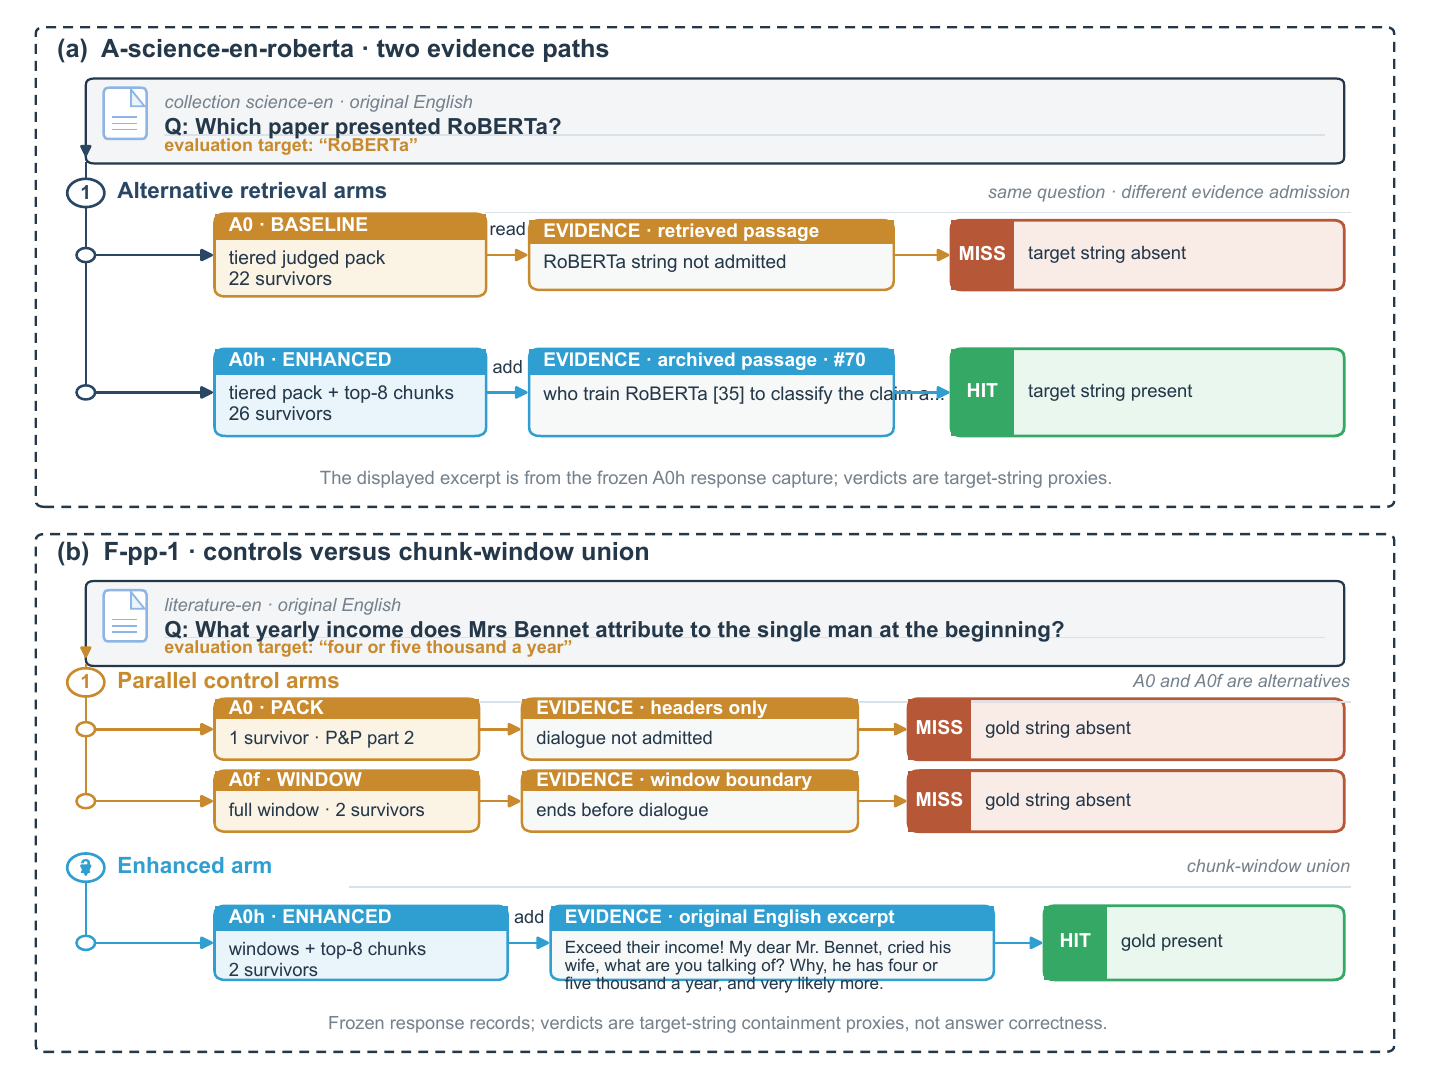
\includegraphics[width=0.58\textwidth]{figs/fig_opt_case.png}
\caption{Two frozen evidence paths. (a) A-science-en-roberta: A0 misses
``RoBERTa,'' whereas A0h admits an archived passage containing it. (b) F-pp-1:
A0 and A0f stop before the dialogue, whereas A0h admits the original excerpt.
HIT/MISS indicates annotated target-string containment in the recorded evidence
pack; a target occurrence may be in a non-gold document, so this is not
gold-document retrieval or semantic answer correctness.}

\end{figure}

\begin{figure}
\centering
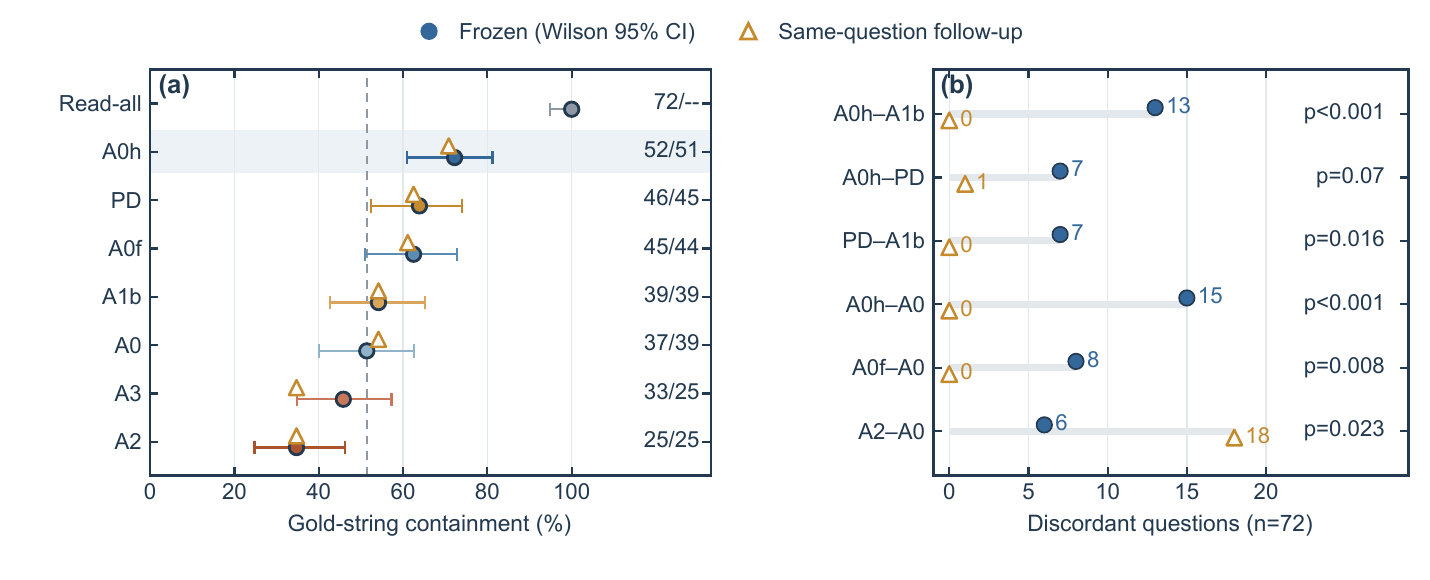
\includegraphics[width=\textwidth]{figs/fig_opt_content.png}
\caption{Content-layer configurations on 72 in-domain questions. (a) Frozen
annotated target-string containment in the returned evidence pack, with Wilson
95\% intervals (filled circles) and the same-question follow-up (open
triangles); counts are in the right-hand column (frozen / follow-up). A
sibling-document occurrence may count; these are lexical proxies, not
 gold-document retrieval or answer correctness. The frozen aggregate combines
dates; A3 was added separately to the follow-up and read-all was incomplete.
The dashed line marks frozen A0. (b) Paired discordance for six frozen
contrasts; each point is the number of questions on which the first (circle)
or second (triangle) arm alone contained the string; $p$ values are two-sided
exact McNemar, unadjusted. A0h, PD and A1b change multiple components; A0,
A1b and A3 may use the gold domain for reference resolution; read-all is a
mechanical scan, not an answering agent.}

\end{figure}


%% n8c_eval.tex — E6 answer behaviour/abstention/cost, E7 deployment arms,
%% E8 verifier failure, E9 operational boundaries.
%% Every figure is attributed to its artefact; corpora are never mixed.
%% LABEL MAP (2026-11-13 renumbering; labels are historical, titles current):
%%   sec:e5 -> E6 | sec:sysarms -> E7 | sec:e6 -> E8 | sec:e7 -> E9
%%   (in n8a: sec:routing-audit -> E3; in n8b: sec:e3 -> E4, sec:ladder-opt -> E5)
%% 2026-11-16: the 30-cell body table moved to supplement S14; E6 now leads
%% with the marker figure (fig_opt_answer) and the layered gold/marker reading.

\subsection{E6: Answer and trace checks, abstention and cost}


Two ten-question grids on the arXiv question set compare a platform agent
(P), direct file tools (F)
and a chunk-replica arm (C) that searches an 800-character chunk copy of the
same content through the platform's own vector lane---a same-content,
flat-chunk substrate control for the document-level organisation. The
original grid uses different substrates; the later grid pins the same five
libraries, and its C arm searches those libraries directly. Gold-ID
presence, strict and alias-aware keyword coverage and citation markers are
deterministic checks, not assessments of semantic support. An identifier in
the trace need not have been read; a marker does not establish that a cited
passage exists or entails the answer. Figure~8 shows the
per-question marker pattern; Table~S14 gives the per-question records and
Table~S15 the aggregate checks and run-time observations.

In both grids the gold identifier occurred in the answer or trace of all 60
cells. Because an identifier in a trace need not have been read, this
identifier-presence check cannot distinguish document reachability; the
observed separation is instead in document-style citation markers. In the
original grid, marker-bearing
answers were 9/10 for P, 7/10 for F and 2/10 for C
(Figure~8a); strict keyword coverage was 9/10 for each arm
and alias-aware coverage 10/10. Under the common substrate, markers were
9/10 in every arm (Figure~8b), strict coverage 7/10, 7/10
and 8/10, and alias-aware coverage 9/10, 9/10 and 10/10. The original-grid
mean time and cost were 52.6 s and $\$0.711$ per question for P, 22.2 s and
$\$0.487$ for F, and 24.5 s and $\$0.527$ for C; these are single-run
observations. Both grids carry a marker in 18 cells and neither in three
(21/30 agreement); the replication adds a marker in nine cells and removes
none (9--0 discordance, McNemar $p=0.0039$), so the marker gap is
substrate-bound rather than an interface
effect alone. The detailed source-presence audit appears in Tables~S7--S8
of the supplementary inventory and is not an entailment test.

A later ten-question run on the repaired platform, with the same five
libraries, returned the gold identifier and a citation marker in all ten
answers, with full keyword coverage in nine (one question covered one of
two annotated terms). Its mean wall-clock was 131 s per question and its
total cost was 3.10 USD. This is a single current-state observation on a
later stack and model state; it is not a controlled arm and is not pooled
with the grids. Read together, the records support a bounded claim:
document-level organisation is associated with document-style citation
behaviour---the tiered platform arm carried markers in 9/10 and, after
repair, 10/10 answers, against 2/10 for the flat chunk replica in the
original grid---but these are lexical proxies; no semantic-quality
superiority is claimed, and the latest run's keyword coverage (9/10) matches
F and trails the historical P arm.

\textbf{Answer-level case study.} A separate recorded demonstration parsed
and ingested a DeepSeek-R1 paper, then used two agent harnesses on the same
four questions. The prompt supplied the library, paper and arXiv identifier
and prescribed the retrieval, judging and reading steps; it did not test
autonomous collection selection. The case compendium reports eight responses
checked against the source on answer content, document provenance, quoted
material and fabricated facts; all eight passed that case review (Table
S16). On the question asking for electricity cost, both responses said the
paper did not provide an electricity figure and distinguished the reported
$\$294$K GPU-rental-based training-cost estimate. This is an observed
refusal to infer an absent value, not a general abstention guarantee. Three
further industrial-corpus probes returned not-found; the retrieval
threshold retained candidates in related absent probes (Fig.~S3).

\begin{figure}
\centering
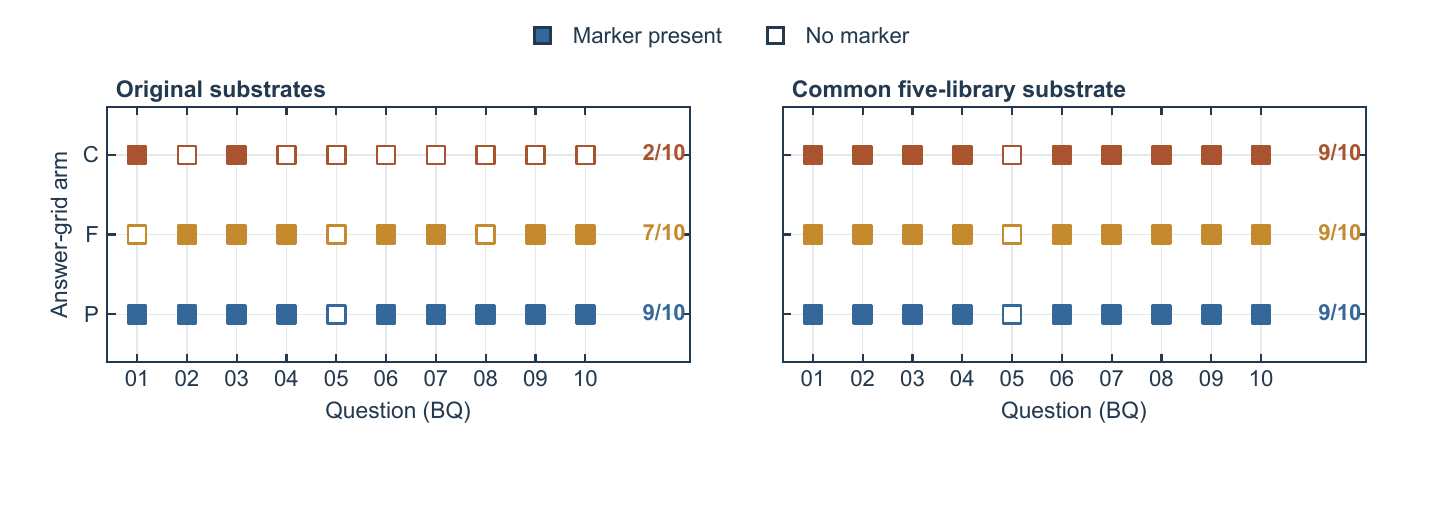
\includegraphics[width=\textwidth]{figs/fig_opt_answer.png}
\caption{Answer traceability on two ten-question grids. (a) Original grid:
rows P, F and C, columns BQ01--BQ10; a filled square marks a document-style
marker and the row-end count is the number of marker-bearing answers
(9/10, 7/10, 2/10). (b) Common-substrate replication on the same five
libraries: markers are 9/10 in every arm. Gold-ID presence is 10/10 in every
cell of both grids; strict keyword coverage is 9/9/9 in (a) and 7/7/8 in
(b); alias-aware coverage is 10/10/10 and 9/9/10. Markers are lexical
proxies and do not verify source resolution or entailment; each arm is one
run, and the original grid uses different substrates. The replication
changes the substrate and raises C and F markers, so the marker gap is not
an interface effect alone.}

\end{figure}
\begin{figure}
\centering
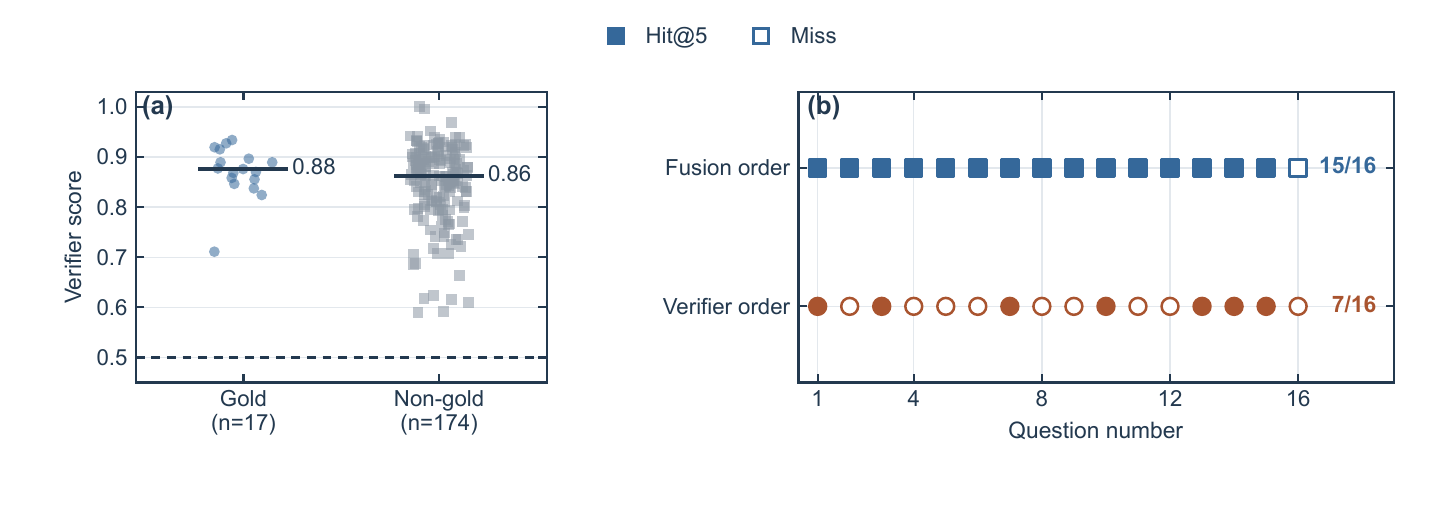
\includegraphics[width=\textwidth]{figs/fig_opt_verifier.png}
\caption{Verifier scores and same-pool ordering. (a) Recorded Laya scores
for 191 candidates from sixteen hybrid runs: 17 in-pool golds and 174
non-golds; all recorded values exceed the 0.5 threshold; one additional Q14
fusion candidate has no recorded score. Horizontal jitter is for legibility;
medians are 0.88 and 0.86; the Mann--Whitney $p=0.26$ is exploratory and
ignores clustering by query. (b) The same sixteen pools replayed with fusion
order and with verifier order; filled squares and circles mark a gold in the
top five, open marks a miss; Hit@5 is 15/16 for fusion order and 7/16 for
verifier order. The score archive and the ordering archive are separate
records. The verifier is not a ranker; these records do not show that
threshold filtering is ineffective or that another verifier would behave
the same way.}

\end{figure}

\subsection{E7: Deployment-layer system arms and honesty contracts}

Three questions crossed pinned, unpinned and pinned hybrid-directed API
arms. The pinned arms returned the two in-corpus gold identifiers, and all
three reported not-found for the out-of-corpus probe. In one unpinned
setting, a 131-document, 74.9 KB catalogue exceeded the tool-output budget;
a truncated preview led to false refusal or a hang. After pagination and
grouped views were added, selected reruns completed, including the formerly
failing query. These observations do not establish general transport
reliability; they show that the management-to-answer path can fail in
transport and that this failure mode is exposed by the workflow rather than
hidden---the silent index-skip fault in E9 is the counterexample that
motivates surfaced degradation markers.
An eighteen-arm honesty battery observed no fabricated citations in its
final responses; interrupted arms were rerun and each arm has one final
observation. The deployment checks are operational boundaries, not a
retrieval comparison.

\subsection{E8: When the verifier fails}


The 191 recorded candidate scores from 16 hybrid runs included 17 in-pool
golds and 174 non-golds. All recorded scores exceeded the 0.5 threshold; one
additional Q14 candidate had no recorded score. Gold and non-gold medians
were 0.88 and 0.86 (Figure~9a). The candidate-level
Mann--Whitney test ($p=0.26$) is exploratory and ignores clustering by
query. The score archive and the ordering archive are separate records.
Re-ranking these scores reduced Hit@5 to 7/16, compared with 15/16 when
recorded survivors retained fusion order (Figure~9b). A Q2
example appears in Fig.~S5: the gold root-cause report scored 0.846 against
five telemetry reports at 0.887--0.926 and was demoted from fusion rank 1 to
rank 8, outside the read window. A replay of the same pairs with an NLI
checkpoint produced Hit@5 0.3125; a span-level replay produced 0.1875. A
relative-margin replay kept 16 of 17 golds at $m=0.15$ and all 17 at
$m=0.20$, while the mean candidate count stayed near twelve; these replays
neither isolate truncation nor establish the cause of verifier failure. The
arXiv corpus did not show the same top-five collapse; domain, language and
corpus size changed together. No answer-level test validates a higher
filtering threshold; Table~S6 of the supplementary inventory sweeps the
recorded scores and Fig.~S4 replays relative-margin variants of the same
pools. The result is a role warning: the verifier can filter, but ordering
by its score lost the gold in this pool. Filtering itself was never
activated, because every recorded score passed the threshold.

\subsection{E9: Operational boundaries: stability, concurrency, gate and
scope ablations}

A 27-cell stability campaign completed without recorded answer errors across
three tasks, three lanes and three rounds. On one instance, a concurrency
sweep of 90/180/270 requests at 5/15/30 clients raised median latency from
5.2 to 1577 ms; 111 of 270 requests timed out at 30 clients. A later cache
repair lowered selected 30-client read-ladder median latency to 65.8 ms,
but the full sweep was not repeated. These are single-instance measurements;
raw concurrent-write counts and crash-recovery evidence were unavailable. A
post-acceptance inspection also exposed a coverage fault mode in the
cross-library vector channel: collections whose on-disk index segments are
unreadable are silently skipped inside the per-collection loop, and the
response still reports success without any degraded marker. Logs identified
eight affected collections in one inspection, including a freshly ingested
library. For that library, a scoped probe found the document while the
global search missed it; forced re-indexing restored the global hit. A
scoped probe on another affected library also returned no results, so the
failure cannot be assumed to be confined to the global channel. Logs surface
the underlying read error, but the response does not; until the repair
ships, coverage claims over the global channel should be read against this
fault mode.

A reconstructed fixed-candidate gate comparison used ten questions, a
12-candidate cap and a 4,000-character pack. All three arms packed the gold
first for the eight gold-answerable questions; for nine of ten questions the
filtered and unfiltered document sets matched. LLM grades still varied under
identical packs (including $0\to5$ and $3\to0$), so these observations do
not establish an answer-quality benefit from gating. The two non-gold
questions, an unanswerable clinical question and an out-of-corpus
particle-physics question, were refused in every arm; the judge-survivor
lists were empty in 2/4 A0 and 0/4 A0h out-of-domain routing probes. Both
A0 empty cases lacked a top candidate; these are retrieval-stage outcomes,
not verified gate rejections or answer-level refusal rates.

The scope diagnostic used ten arXiv questions, eight of which had gold
documents in the evaluation corpus; the other two were excluded from Hit@5.
With the gold library pinned, Hit@5 was 1.0 on the eight graded questions;
pinning a non-gold library yielded 0.0. The unscoped search covered 20 live
libraries, including 15 outside the five-library evaluation corpus, and is
not a matched-scope comparison. The catalogue route selected the correct
library first for six of eight answerable questions; file names carried
domain prefixes. These small, single-engine experiments do not establish an
independent effect of content placement or an overall system advantage;
they define the operational envelope in which the management and answer
results should be read.


\section{Discussion and lessons learned}


The management evidence is the first result, not merely a precondition for the
retrieval experiments. Across the acquisition and organisation campaigns, HMRS
recorded 322 stored parts across five libraries, measured content-based
assignment separately from retrieval, and exposed state disagreement after a
rename and in selected lifecycle checks. The 79/21 arXiv availability result
and the 0.875/1.0/1.0 cross-lingual assignment result come from different
corpora and should be read as complementary evidence: the former identifies an
incomplete ingestion boundary, while the latter tests content-based placement.
The 33-part consistency sample and selected passing lifecycle checks show
that the management loop is exercisable, not that it is transactionally
complete. The failed task-status/update checks and stale-index rename are
important system results because they show why reconciliation and post-operation
probes are part of the design rather than optional diagnostics.

The access results then show how managed state is consumed. The frozen route-card
audit selected the gold collection in 72/72 full-card cases and 37/72 nominally
name-only cases, but its fallback and scripted nature prevent a causal
interpretation. In the latest complete R3 content-layer follow-up on the same
questions, A0h, the tiered configuration with a chunk-window union, had the
highest observed annotated target-string containment in returned evidence packs
at 51/72 questions; a sibling-document occurrence may count. PD, A0f, A0/A1b and A2 contained it in
45/72, 44/72, 39/72 and 25/72, respectively. A0h versus A0 was 12--0
($p=0.00049$, exploratory and unadjusted). These are containment proxies, not
semantic answers, and the configurations vary in more than navigation alone.
The frozen read-all scan found every string but generated no answers, while the
R3 read-all run was incomplete; this is why the mechanical upper bound is not a
current Agent baseline. These observations describe the tested configuration
on this corpus and question set; they do not establish a universal advantage of hierarchical
retrieval.

The same-pool diagnostic illustrates how candidate-evidence ordering can matter
in this setting. On identical logged pools from the retired hybrid wrapper,
verifier-score ordering reproduced the Hit@5 collapse documented in
Section~8.9; all 191 recorded scores exceeded the configured
threshold, so filtering did not activate and its benefit was not measured.
This is a bounded warning about a particular ordering, not a finding about
every verifier or current retrieval lane.

The reported answer and refusal cases show selected workflow behaviour, not a
reliable abstention rate. Pagination repaired selected oversized catalogue
paths, but incomplete searches and tool failures remain distinct from a
completed search without support. A late inspection also found that the global
channel can silently skip unreadable library indexes while reporting success;
until this is surfaced, a successful response is not evidence of complete
cross-library coverage. The inspection identified eight affected collections;
scoped search worked for the newly ingested example, but a probe on another
affected library returned no results. Stronger claims need
independent questions, controlled single-factor comparisons, repeated runs,
semantic support review, and tests of operations and recovery beyond the
present local setting.


\section{Threats to validity}


\noindent\textbf{Data and scope.} The corpora and questions are small and
bounded; questions and gold annotations were developer-authored. The
management campaigns and the access campaigns use different corpora and
should not be pooled. The 72-question route set includes 52 automatically
expanded questions, and 47 questions come from three English domains. Four
out-of-domain probes cannot estimate abstention rates. The storage
reconciliation checks 33 of 322 parts. Different retrieval arms use different
scopes or substrates; the historical hybrid wrapper, not the current composed
hybrid lane, was tested. Broader generalisation requires independent questions,
larger corpora and matched single-factor comparisons across the content-layer
configurations.

\noindent\textbf{Measurement and comparisons.} Annotated target-string
containment in a returned evidence pack is a substring proxy, not gold-document
retrieval, semantic answer correctness or entailment; a sibling-document
occurrence may count. Gold-ID, lexical and citation marker checks likewise do
not establish claim-to-source support. Two answer
grids used ten questions, one model and one run per arm; one replication held
libraries fixed, while substrates differed in the original grid. The scripted
full-read baseline searches strings and generates no answer. A0h, A1b and PD
change multiple components, and A0, A1b and A3 may use the gold domain to
resolve candidate references. Historical traces do not quantify this fallback.
A3 can also admit candidates outside the evaluated libraries and its
name-only routing may fall back to descriptions. Thus these arms cannot isolate
navigation or establish deployed performance. The later run repeats the same
questions and is not an independent test set; code hashes and judge inputs are
not fully preserved for each historical record.

\noindent\textbf{Statistical and operational validity.} Paired tests are
exploratory and not pre-registered; Wilson intervals condition on the sampled
questions and do not capture run-to-run variance. Candidate- and span-level
tests treat observations within queries as independent and may be
anti-conservative. Some E5 reference-mode score and candidate inputs were not retained; the E8
verifier replay is reproducible from the released scores, golds and grader.
The manual refusal battery has one final observation per arm, and experience
approval was not exercised. The 16 lifecycle assertions, selected pagination
checks and one-workstation concurrency measurements do not establish multi-host
reliability, adversarial security, human adoption or crash recovery. The global
cross-library vector channel also silently skipped unreadable collections in
one inspection while reporting success; until the response exposes this
condition, successful global queries do not establish complete corpus coverage.
Future work should instrument the reference lookup, remove gold-dependent
fallback, conduct matched single-factor ablations and a genuine agent full-read
baseline, surface global-channel degradation, and pre-specify repeated
comparisons and multiplicity control.


\section{Conclusion}


HMRS is a knowledge-document management system whose retrieval path depends on
managed state. It parses heterogeneous sources, assigns content to collections,
derives descriptions and tags, stores documents and structural parts, exposes
catalogue-first access, and records lifecycle state across document files, the
tree registry and per-library metadata. The segment-level gate adds provenance
and an admission signal; it is not a truth oracle or a ranker. This separation
of managed objects, access views and workflow decisions is the system's central
design claim.

The management campaigns show that this loop is operational but not complete.
The 100-paper arXiv campaign produced 322 parts, with 79 papers retrievable and
21 not; the separate 400-pages-per-language test measured content-based
assignment accuracy of 0.875 for English and 1.0 for Chinese and Japanese. A
33-part storage sample passed its selected checks, while a rename exposed stale
index state and 16 lifecycle scenarios included failures in task-status and
update checks. The system therefore contributes a testable management loop with
explicit failure visibility, rather than an unqualified claim of automatic
consistency.

The access campaigns provide the next layer of evidence. The frozen route-card
audit produced 72/72 full-card versus 37/72 nominally name-only collection
selection, with an unlogged fallback that prevents causal attribution. In the
latest complete R3 content-layer follow-up on the same questions, the tiered
chunk-window arm A0h achieved 51/72 (70.8\%), above PD 45/72, A0f 44/72, A0/A1b 39/72 and A2 25/72; its paired
contrast with A0 was 12--0 ($p=0.00049$, exploratory). A0h was the highest
configuration in the frozen run, an archived reproduction and the follow-up,
with the A0h $>$ PD $>$ A0f ordering preserved in all three; A1b and A2
repeated their frozen counts exactly. These values are annotated target-string containment proxies in returned
evidence packs; a sibling-document occurrence may count, and the arms vary in
more than navigation.
The frozen read-all script found all 72 strings but generated no answers, and
R3 read-all was incomplete. At the answer layer, gold identifiers appeared in
all 60 grid cells and in a later ten-question run; document-style citation
markers separated the substrates (9/7/2, then 9/9/9 on a common substrate,
and 10/10 after repair against the flat chunk replica's 2/10; the last
pairing is cross-run and is not pooled)---lexical
contrasts, not semantic support. Together, the results support the narrower
claim that A0h had the highest observed annotated target-string containment in
returned evidence packs among completed arms on this corpus and question set,
not gold-document retrieval, semantic answer accuracy, universal retrieval
superiority or a single-factor causal hierarchy claim.

These bounded results support treating the collection as a managed, auditable
object and motivate its use as an inspectable basis for evidence-traced
retrieval. The immediate deployment implication is to expose collection state
and incomplete paths, retain evidence provenance, and separately evaluate
verifier-based admission and ordering before deployment. The global channel can also
silently skip unreadable library indexes while reporting success; until that
condition is surfaced, a successful cross-library response is not evidence of
complete coverage. The study's contribution is a system-level management
contract and a bounded A0h observation, not a claim of universal retrieval
superiority. Broader evaluation needs semantic support review, independently
authored questions, repeated agent trials with run-to-run variance estimates,
larger matched comparisons with multiplicity control, and crash-recovery tests.


%% n_back.tex — back matter, included by main_20p.tex after n11_conclusion.tex
%% and before the bibliography. This file is the single source of truth for
%% every declaration; n11_conclusion.tex carries the Conclusion and nothing else.
%%
%% The declarations follow the Conclusion. Keep the generative-AI statement
%% immediately before the references, pending a final check of the current KBS
%% Guide for Authors.
%%
%% AUTHOR ACTION: replace the CRediT names, confirm the funding wording, and
%% adjust or remove the acknowledgements.

\section*{CRediT authorship contribution statement}
\textbf{Author 1:} Conceptualisation, Methodology, Software, Investigation,
Data curation, Writing -- original draft. \textbf{Author 2:} Validation,
Writing -- review \& editing, Supervision. %% AUTHOR ACTION: adjust.

\section*{Declaration of competing interest}
The authors declare that they have no known competing financial interests
or personal relationships that could have appeared to influence the work
reported in this paper.

\section*{Funding}
This research did not receive any specific grant from funding agencies in
the public, commercial, or not-for-profit sectors. %% AUTHOR ACTION

\section*{Ethics statement}
This article does not report studies involving human participants, human
data, or animals.

\section*{Data availability}
Source code and benchmark scripts are available at
\url{https://github.com/kingdol666/rag-knowledge}. The repository indexes the
artefact inventory; hashes for the corrected and pre-correction annotations
and grader are recorded in
\path{paper-kbs/tex/journal_20p/revision-20261112.sha256}.
The supplement contains campaign inventories, per-question summaries and
lifecycle and ablation tables. De-identified per-question records for the
November 2026 route and content-layer campaigns are prepared for deposit
alongside the supplement (frozen, follow-up and floor trace CSVs); each row
carries the arm, question identifier, containment outcome, byte and timing
totals and, where applicable, route labels. Question texts, gold strings and
evidence-pack contents are withheld because of source-document restrictions.
The CSV files and revision manifest must be included in the deposited package
before submission.
The 42-document industrial corpus is a non-customer demonstration instance,
not deposited publicly. The verifier comparison is reproducible from the
released scores, golds and grader; an end-to-end rerun needs a substitute
corpus, with a recipe and synthetic sample in
\path{paper-kbs/notes/industrial-corpus-substitute-recipe-2026-10-16.md}.

\section*{Acknowledgments}
The authors thank the maintainers of the open-source components the platform
builds on. %% AUTHOR ACTION: adjust or remove.

%% AUTHOR ACTION: confirm all service names and versions before submission.
\section*{Declaration of generative AI and AI-assisted technologies in the manuscript preparation process}
The authors used Anthropic Claude Code, ZCode, OpenAI Codex and an AI image
generation tool for experiment execution, tabulation, language editing and
initial figure design. The authors reviewed the final text and figures and take
responsibility for them; all reported experimental numbers come from logged
runs on the authors' machine.



\section*{References}




[1] 
Y.~Gao, Y.~Xiong, M.~Wang, H.~Wang, Modular {RAG}: Transforming {RAG} systems
  into {LEGO}-like reconfigurable frameworks, ACM Transactions on Information
  Systems 44 (2026) 1--53.
  doi:10.1145/3837856.



[2] 
Y.~Gao, Y.~Xiong, X.~Gao, et~al., Retrieval-augmented generation for large
  language models: A survey, arXiv preprint arXiv:2312.10997 (2023).
  doi:10.48550/arXiv.2312.10997.



[3] 
P.~Lewis, E.~Perez, A.~Piktus, F.~Petroni, V.~Karpukhin, N.~Goyal,
  H.~K{\"u}ttler, M.~Lewis, W.~Yih, T.~Rockt{\"a}schel, S.~Riedel, D.~Kiela,
  \href{https://proceedings.neurips.cc/paper/2020/hash/6b493230205f780e1bc26945df7481e5-Abstract.html}{Retrieval-augmented
  generation for knowledge-intensive {NLP} tasks}, in: Advances in Neural
  Information Processing Systems, Vol.~33, Curran Associates, Inc., 2020, pp.
  9459--9474.
\newlinehttps://proceedings.neurips.cc/paper/2020/hash/6b493230205f780e1bc26945df7481e5-Abstract.html



[4] 
V.~Karpukhin, B.~O{\u{g}}uz, S.~Min, P.~Lewis, L.~Wu, S.~Edunov, D.~Chen,
  W.~Yih, Dense passage retrieval for open-domain question answering, in:
  Proceedings of the 2020 Conference on Empirical Methods in Natural Language
  Processing ({EMNLP}), 2020, pp. 6769--6781.
  doi:10.18653/v1/2020.emnlp-main.550.



[5] 
{Model Context Protocol Contributors}, Model context protocol specification
  (2025-11-25), https://modelcontextprotocol.io/specification/2025-11-25,
  accessed September 19, 2026; specification revision 2025-11-25 (2025).



[6] 
A.~Singh, A.~Ehtesham, S.~Kumar, T.~T. Khoei, A.~V. Vasilakos, Agentic
  retrieval-augmented generation: A survey on agentic {RAG}, arXiv preprint
  arXiv:2501.09136 (2025).
  doi:10.48550/arXiv.2501.09136.



[7] 
S.~Robertson, H.~Zaragoza, The probabilistic relevance framework: {BM25} and
  beyond, Foundations and Trends in Information Retrieval 3~(4) (2009)
  333--389.
  doi:10.1561/1500000019.



[8] 
G.~V. Cormack, C.~L.~A. Clarke, S.~Buettcher, Reciprocal rank fusion
  outperforms {Condorcet} and individual rank learning methods, in: Proceedings
  of the 32nd International {ACM} {SIGIR} Conference on Research and
  Development in Information Retrieval, 2009, pp. 758--759.
  doi:10.1145/1571941.1572114.



[9] 
D.~Edge, H.~Trinh, N.~Cheng, J.~Bradley, A.~Chao, A.~Mody, S.~Truitt,
  D.~Metropolitansky, R.~O. Ness, J.~Larson,
  \href{https://arxiv.org/abs/2404.16130}{From local to global: A {GraphRAG}
  approach to query-focused summarization}, arXiv preprint arXiv:2404.16130
  (2024).
\newlinehttps://arxiv.org/abs/2404.16130



[10] 
Z.~Guo, L.~Xia, Y.~Yu, T.~Ao, C.~Huang, {LightRAG}: Simple and fast
  retrieval-augmented generation, in: Findings of the Association for
  Computational Linguistics: EMNLP 2025, 2025, pp. 10746--10761.
  doi:10.18653/v1/2025.findings-emnlp.568.



[11] 
P.~Sarthi, S.~Abdullah, A.~Tuli, S.~Khanna, A.~Goldie, C.~D. Manning, {RAPTOR}:
  Recursive abstractive processing for tree-organized retrieval, in: The
  Twelfth International Conference on Learning Representations ({ICLR}), 2024.
  doi:10.48550/arXiv.2401.18059.



[12] 
T.~P{\"a}iv{\"a}rinta, B.~E. Munkvold, Enterprise content management: An
  integrated perspective on information management, in: Proc. 38th Annual
  Hawaii International Conference on System Sciences (HICSS), IEEE, 2005, pp.
  96--96.
  doi:10.1109/hicss.2005.244.



[13] 
P.~Tyrv{\"a}inen, T.~P{\"a}iv{\"a}rinta, A.~Salminen, J.~Iivari, Characterizing
  the evolving research on enterprise content management, European Journal of
  Information Systems 15~(6) (2006) 627--634.
  doi:10.1057/palgrave.ejis.3000648.



[14] 
J.-R. Park, Metadata quality in digital repositories: A survey of the current
  state of the art, Cataloging \& Classification Quarterly 47~(3-4) (2009)
  213--228.
  doi:10.1080/01639370902737240.



[15] 
S.~A. Golder, B.~A. Huberman, Usage patterns of collaborative tagging systems,
  Journal of Information Science 32~(2) (2006) 198--208.
  doi:10.1177/0165551506062337.



[16] 
S.~Auer, C.~Bizer, G.~Kobilarov, J.~Lehmann, R.~Cyganiak, Z.~Ives, {DBpedia}: A
  nucleus for a web of open data, in: The Semantic Web (ISWC/ASWC 2007),
  Lecture Notes in Computer Science, Springer, 2007, pp. 722--735.
  doi:10.1007/978-3-540-76298-0_52.



[17] 
J.~Hoffart, F.~M. Suchanek, K.~Berberich, G.~Weikum, {YAGO2}: A spatially and
  temporally enhanced knowledge base from {Wikipedia}, Artificial Intelligence
  194 (2013) 28--61.
  doi:10.1016/j.artint.2012.06.001.



[18] 
Y.~Zhang, Y.~Li, L.~Cui, D.~Cai, L.~Liu, T.~Fu, X.~Huang, E.~Zhao, Y.~Zhang,
  C.~Xu, Y.~Chen, L.~Wang, A.~T. Luu, W.~Bi, F.~Shi, S.~Shi,
  \href{https://arxiv.org/abs/2309.01219}{Siren's song in the {AI} ocean: A
  survey on hallucination in large language models}, arXiv preprint
  arXiv:2309.01219 (2023).
\newlinehttps://arxiv.org/abs/2309.01219



[19] 
J.~P. Callan, Z.~Lu, W.~B. Croft, Searching distributed collections with
  inference networks, in: Proc. of the 18th Annual International ACM SIGIR
  Conference (SIGIR '95), 1995, pp. 21--28.
  doi:10.1145/215206.215328.



[20] 
L.~Si, J.~Callan, Relevant document distribution estimation method for resource
  selection, in: Proc. of the 26th Annual International ACM SIGIR Conference
  (SIGIR '03), 2003, pp. 298--305.
  doi:10.1145/860435.860490.



[21] 
W.~Yang, L.~Some, M.~Bain, B.~Kang, A comprehensive survey on integrating large
  language models with knowledge-based methods, Knowledge-Based Systems 318
  (2025) 113503.
  doi:10.1016/j.knosys.2025.113503.



[22] 
I.~Nonaka, A dynamic theory of organizational knowledge creation, Organization
  Science 5~(1) (1994) 14--37.
  doi:10.1287/orsc.5.1.14.



[23] 
I.~Nonaka, R.~Toyama, N.~Konno, {SECI}, {Ba} and leadership: a unified model of
  dynamic knowledge creation, Long Range Planning 33~(1) (2000) 5--34.
  doi:10.1016/s0024-6301(99)00115-6.



[24] 
E.~Mosqueira-Rey, E.~Hern{\'a}ndez-Pereira, D.~Alonso-R{\'i}os,
  J.~Bobes-Bascar{\'a}n, {\'A}.~Fern{\'a}ndez-Leal, Human-in-the-loop machine
  learning: a state of the art, Artificial Intelligence Review 56~(4) (2022)
  3005--3054.
  doi:10.1007/s10462-022-10246-w.



[25] 
A.~Barredo~Arrieta, N.~D{\'i}az-Rodr{\'i}guez, J.~Del~Ser, A.~Bennetot,
  S.~Tabik, A.~Barbado, S.~Garcia, S.~Gil-Lopez, D.~Molina, R.~Benjamins,
  R.~Chatila, F.~Herrera, Explainable artificial intelligence ({XAI}):
  Concepts, taxonomies, opportunities and challenges toward responsible {AI},
  Information Fusion 58 (2020) 82--115.
  doi:10.1016/j.inffus.2019.12.012.



[26] 
F.~Sebastiani, Machine learning in automated text categorization, ACM Computing
  Surveys 34~(1) (2002) 1--47.
  doi:10.1145/505282.505283.



[27] 
X.~Zhong, J.~Tang, A.~Jimeno~Yepes, {PubLayNet}: Largest dataset ever for
  document layout analysis, in: 2019 International Conference on Document
  Analysis and Recognition (ICDAR), IEEE, 2019, pp. 1015--1022.
  doi:10.1109/icdar.2019.00166.



[28] 
Y.~Huang, T.~Lv, L.~Cui, Y.~Lu, F.~Wei, {LayoutLMv3}: Pre-training for document
  {AI} with unified text and image masking, in: Proc. 30th ACM International
  Conference on Multimedia (MM '22), ACM, 2022, pp. 4083--4091.
  doi:10.1145/3503161.3548112.



[29] 
B.~Wang, C.~Xu, X.~Zhao, L.~Ouyang, F.~Wu, Z.~Zhao, R.~Xu, K.~Liu, Y.~Qu,
  F.~Shang, B.~Zhang, L.~Wei, Z.~Sui, W.~Li, B.~Shi, Y.~Qiao, D.~Lin, C.~He,
  {MinerU}: An open-source solution for precise document content extraction,
  arXiv preprint arXiv:2409.18839 (2024).
  doi:10.48550/arXiv.2409.18839.



[30] 
G.~S. Manku, A.~Jain, A.~Das~Sarma, Detecting near-duplicates for web crawling,
  in: Proc. 16th International Conference on World Wide Web (WWW '07), ACM,
  2007, pp. 141--150.
  doi:10.1145/1242572.1242592.



[31] 
P.~Missier, K.~Belhajjame, J.~Cheney, The {W3C} {PROV} family of specifications
  for modelling provenance metadata, in: Proc. 16th International Conference on
  Extending Database Technology (EDBT/ICDT '13), ACM, 2013, pp. 773--776.
  doi:10.1145/2452376.2452478.



[32] 
J.~Cheney, L.~Chiticariu, W.-C. Tan, Provenance in databases: Why, how, and
  where, Foundations and Trends in Databases 1~(4) (2009) 379--474.
  doi:10.1561/1900000006.



[33] 
M.~G. Oca{\~n}a, A.~L. Opdahl, {A Software Reference Architecture for
  Journalistic Knowledge Platforms}, Knowledge-Based Systems 276 (2023) 110750.
  doi:10.1016/j.knosys.2023.110750.



[34] 
M.~Gallofr\'e Oca\~na, A.~L. Opdahl, Developing a software reference
  architecture for journalistic knowledge platforms, in: Proceedings of the 6th
  Workshop on Semantic Access to Big Data and AI (SAML), Vol. 2978 of CEUR
  Workshop Proceedings, 2021.



[35] 
Y.~Yang, H.~Huang, Y.~Gao, J.~Li, {Building knowledge-grounded dialogue systems
  with graph-based semantic modelling}, Knowledge-Based Systems 298 (2024)
  111943.
  doi:10.1016/j.knosys.2024.111943.



[36] 
E.~Budur, R.~{\"O}z{\c{c}}elik, D.~Soylu, O.~Khattab, T.~G{\"u}ng{\"o}r,
  C.~Potts, {Building efficient and effective OpenQA systems for low-resource
  languages}, Knowledge-Based Systems 302 (2024) 112243.
  doi:10.1016/j.knosys.2024.112243.



[37] 
G.~D. Vito, F.~Ferrucci, A.~Angelakis, {HELIOT: LLM-Based CDSS for adverse drug
  reaction management}, Knowledge-Based Systems 328 (2025) 114184.
  doi:10.1016/j.knosys.2025.114184.



[38] 
I.~Aarab, {LLM-based IR-system for bank supervisors}, Knowledge-Based Systems
  310 (2024) 112914.
  doi:10.1016/j.knosys.2024.112914.



[39] 
X.~Liao, Y.~Mao, W.~Liu, A.~Yang, {A practical and privacy-preserving framework
  for real-world large language model services}, Knowledge-Based Systems 337
  (2026) 115347.
  doi:10.1016/j.knosys.2026.115347.



[40] 
E.~C. Garrido-Merch{\'a}n, C.~Puente, {GOFAI meets generative AI: Development
  of expert systems by means of large language models}, Knowledge-Based Systems
  351 (2026) 116657.
  doi:10.1016/j.knosys.2026.116657.



[41] 
S.~Hou, A.~Zhao, J.~Liang, Z.~Shen, H.~Wu, {Geo-FuB: A method for constructing
  an Operator-Function knowledge base for geospatial code generation with large
  language models}, Knowledge-Based Systems 319 (2025) 113624.
  doi:10.1016/j.knosys.2025.113624.



[42] 
G.~Ciatto, A.~Agiollo, M.~Magnini, A.~Omicini, {Large language models as
  oracles for instantiating ontologies with domain-specific knowledge},
  Knowledge-Based Systems 310 (2025) 112940.
  doi:10.1016/j.knosys.2024.112940.



[43] 
A.~H. Mohamed, K.~S. Shalaby, A.~Kaladharan, S.~Sen, H.~Ata{\c{s}}, A.~T.
  Kodamullil, {KG-Orchestra: An Open-Source Multi-Agent Framework for
  Evidence-Based Biomedical Knowledge Graphs Enrichment}, Knowledge-Based
  Systems (2026) 117316doi:10.1016/j.knosys.2026.117316.



[44] 
Y.~Liu, Z.~Abulawi, A.~Garimidi, D.~Lim, {Automating data-driven modeling and
  analysis for engineering applications using large language model agents},
  Knowledge-Based Systems 343 (2026) 115989.
  doi:10.1016/j.knosys.2026.115989.



[45] 
L.-L. Chen, W.~Sun, H.~Xie, Y.~Cai, Y.~Zhang, {Enhancing large language
  model-based systems for end-to-end circuit analysis problem solving},
  Knowledge-Based Systems 353 (2026) 117171.
  doi:10.1016/j.knosys.2026.117171.



[46] 
A.~G. Sorokin, X.~Zhu, E.~H. Lee, B.~Cheng, {SigOpt Mulch: An intelligent
  system for AutoML of gradient boosted trees}, Knowledge-Based Systems 273
  (2023) 110604.
  doi:10.1016/j.knosys.2023.110604.



[47] 
M.-K. Ghali, A.~Farrag, D.~Won, Y.~Jin, Enhancing knowledge retrieval with
  in-context learning and semantic search through generative {AI},
  Knowledge-Based Systems 311 (2025) 113047.
  doi:10.1016/j.knosys.2025.113047.



[48] 
J.~Chen, S.~Xiao, P.~Zhang, K.~Luo, D.~Lian, Z.~Liu, {M3-Embedding}:
  Multi-linguality, multi-functionality, multi-granularity text embeddings
  through self-knowledge distillation, in: Findings of the Association for
  Computational Linguistics: ACL 2024, Association for Computational
  Linguistics, 2024, pp. 2318--2335.
  doi:10.18653/v1/2024.findings-acl.137.



[49] 
F.~Li, X.~Li, J.~Bao, Recursive multi-modal retrieval for structured semantic
  trees in engineering documents, Knowledge-Based Systems 338 (2026) 115433.
  doi:10.1016/j.knosys.2026.115433.



[50] 
A.~Singh, S.~J. Subramanya, R.~Krishnaswamy, H.~V. Simhadri, Freshdiskann: A
  fast and accurate graph-based ann index for streaming similarity search
  (2021).
  arXiv:2105.09613.



[51] 
Y.~Xu, H.~Liang, J.~Li, S.~Xu, Q.~Chen, Q.~Zhang, C.~Li, Z.~Yang, F.~Yang,
  Y.~Yang, P.~Cheng, M.~Yang, Spfresh: Incremental in-place update for
  billion-scale vector search, in: Proc. of the 29th Symposium on Operating
  Systems Principles (SOSP '23), 2023, pp. 545--561.
  doi:10.1145/3600006.3613166.



[52] 
T.~Chen, H.~Wang, S.~Chen, W.~Yu, K.~Ma, X.~Zhao, H.~Zhang, D.~Yu, Dense x
  retrieval: What retrieval granularity should we use?, in: Proc. of EMNLP
  2024, 2024, pp. 15159--15177.
  doi:10.18653/v1/2024.emnlp-main.845.



[53] 
M.~G{\"u}nther, I.~Mohr, D.~J. Williams, B.~Wang, H.~Xiao, Late chunking:
  Contextual chunk embeddings using long-context embedding models (2024).
  arXiv:2409.04701.



[54] 
J.~Shen, H.~Zhu, B.~Zhang, Toward trustworthy engineering information
  extraction using retrieval-augmented generation, Knowledge-Based Systems 348
  (2026) 116418.
  doi:10.1016/j.knosys.2026.116418.



[55] 
S.~Yao, J.~Zhao, D.~Yu, N.~Du, I.~Shafran, K.~Narasimhan, Y.~Cao, {ReAct}:
  Synergizing reasoning and acting in language models, in: The Eleventh
  International Conference on Learning Representations ({ICLR}), 2023.
  doi:10.48550/arXiv.2210.03629.



[56] 
T.~Schick, J.~Dwivedi-Yu, R.~Dess{\`i}, R.~Raileanu, M.~Lomeli, E.~Hambro,
  L.~Zettlemoyer, N.~Cancedda, T.~Scialom, Toolformer: Language models can
  teach themselves to use tools, in: Advances in Neural Information Processing
  Systems, Vol.~36, 2023, pp. 68539--68551.
  doi:10.52202/075280-2997.



[57] 
Z.~Li, H.~Tian, L.~Luo, Y.~Cao, P.~Luo, {DeepRead}: Document structure-aware
  reasoning to enhance agentic search, arXiv preprint arXiv:2602.05014v3
  (2026).
  doi:10.48550/arXiv.2602.05014.



[58] 
L.~Siddharth, J.~Luo, {Retrieval augmented generation using engineering design
  knowledge}, Knowledge-Based Systems 303 (2024) 112410.
  doi:10.1016/j.knosys.2024.112410.



[59] 
Z.~Peng, X.~Wu, Q.~Wang, Y.~Fang, {Soft prompt tuning for augmenting dense
  retrieval with large language models}, Knowledge-Based Systems 309 (2024)
  112758.
  doi:10.1016/j.knosys.2024.112758.



[60] 
L.~Massai, {Evaluation of semantic relations impact in query expansion-based
  retrieval systems}, Knowledge-Based Systems 283 (2023) 111183.
  doi:10.1016/j.knosys.2023.111183.



[61] 
D.~Zan, B.~Chen, Y.~Gong, J.~Cao, F.~Zhang, B.~Wu, B.~Guan, Y.~Yin, Y.~Wang,
  {Private-library-oriented code generation with large language models},
  Knowledge-Based Systems 326 (2025) 113934.
  doi:10.1016/j.knosys.2025.113934.



[62] 
X.~Dai, Y.~Hua, T.~Wu, S.~Yang, J.~Qiu, G.~Qi, {Large language models can
  better understand knowledge graphs than we thought}, Knowledge-Based Systems
  312 (2025) 113060.
  doi:10.1016/j.knosys.2025.113060.



[63] 
W.~Huang, G.~Zhou, M.~Lapata, P.~Vougiouklis, S.~Montella, J.~Z. Pan,
  {Prompting large language models with knowledge graphs for question answering
  involving long-tail facts}, Knowledge-Based Systems 324 (2025) 113648.
  doi:10.1016/j.knosys.2025.113648.



[64] 
D.~Tao, C.~Wang, F.~Huang, J.~Chen, Y.~Huang, M.~Jiang, {Fine-grained Stateful
  Knowledge Exploration: Effective and efficient graph retrieval with Large
  Language Models}, Knowledge-Based Systems 326 (2025) 114011.
  doi:10.1016/j.knosys.2025.114011.



[65] 
A.~Sinha, C.~Agarwal, P.~Malo, {FinBloom: Knowledge-Grounding Large Language
  Model with Real-Time Financial Data}, Knowledge-Based Systems 339 (2026)
  115559.
  doi:10.1016/j.knosys.2026.115559.



[66] 
S.~Saadaoui, E.~Alonso, {Coordinated LLM multi-agent systems for collaborative
  question-answer generation}, Knowledge-Based Systems 330 (2025) 114627.
  doi:10.1016/j.knosys.2025.114627.



[67] 
C.~Packer, S.~Wooders, K.~Lin, V.~Fang, S.~G. Patil, I.~Stoica, J.~E. Gonzalez,
  {MemGPT}: Towards {LLMs} as operating systems, arXiv preprint
  arXiv:2310.08560 (2023).



[68] 
P.~Chhikara, D.~Khant, S.~Aryan, T.~Singh, D.~Yadav, Mem0: Building
  production-ready {AI} agents with scalable long-term memory, arXiv preprint
  arXiv:2504.19413 (2025).



[69] 
W.~Xu, Z.~Liang, K.~Mei, H.~Gao, J.~Tan, Y.~Zhang, {A-MEM}: Agentic memory for
  {LLM} agents, arXiv preprint arXiv:2502.12110 (2025).



[70] 
R.~Wu, K.~Huang, H.~Zhang, Q.~Liu, J.~Guo, J.~Deng, F.~Ye,
  {Information-Theoretic Dual Memory System for continual learning},
  Knowledge-Based Systems 325 (2025) 113913.
  doi:10.1016/j.knosys.2025.113913.



[71] 
A.~Miles, S.~Bechhofer, {SKOS} simple knowledge organization system reference,
  W3C Recommendation, https://www.w3.org/TR/skos-reference/ (2009).



[72] 
A.~Asai, Z.~Wu, Y.~Wang, A.~Sil, H.~Hajishirzi,
  \href{https://openreview.net/forum?id=hSyW5go0v8}{{Self-RAG}: Learning to
  retrieve, generate, and critique through self-reflection}, in: The Twelfth
  International Conference on Learning Representations ({ICLR}), 2024.
\newlinehttps://openreview.net/forum?id=hSyW5go0v8



[73] 
S.-Q. Yan, J.-C. Gu, Y.~Zhu, Z.-H. Ling, Corrective retrieval augmented
  generation, arXiv preprint arXiv:2401.15884 (2024).
  doi:10.48550/arXiv.2401.15884.



[74] 
Z.~Jiang, F.~Xu, L.~Gao, Z.~Sun, Q.~Liu, J.~Dwivedi-Yu, Y.~Yang, J.~Callan,
  G.~Neubig, Active retrieval augmented generation, in: Proceedings of the 2023
  Conference on Empirical Methods in Natural Language Processing ({EMNLP}),
  2023, pp. 7969--7992.
  doi:10.18653/v1/2023.emnlp-main.495.



[75] 
A.~Kamath, R.~Jia, P.~Liang, Selective question answering under domain shift,
  in: Proceedings of the 58th Annual Meeting of the Association for
  Computational Linguistics ({ACL}), 2020, pp. 5684--5696.
  doi:10.18653/v1/2020.acl-main.503.



[76] 
S.~Feng, W.~Shi, Y.~Wang, et~al., Don't hallucinate, abstain: Identifying {LLM}
  knowledge gaps via multi-{LLM} collaboration, in: Proceedings of the 62nd
  Annual Meeting of the Association for Computational Linguistics (ACL), 2024,
  pp. 14664--14690.
  doi:10.18653/v1/2024.acl-long.786.



[77] 
Z.~Yin, Q.~Sun, Q.~Guo, et~al., Do large language models know what they don't
  know?, in: Findings of the Association for Computational Linguistics: ACL
  2023, 2023, pp. 8653--8665.
  doi:10.18653/v1/2023.findings-acl.551.



[78] 
C.~Zhao, R.~{De Maria}, T.~Kumarage, K.~S. Chaudhary, G.~Agrawal, Y.~Li,
  J.~Park, Y.-C. Chen, Y.~Deng, H.~Liu, {CyberBOT}: Ontology-grounded retrieval
  augmented generation for reliable cybersecurity education, in: Proceedings of
  the 34th ACM International Conference on Information and Knowledge
  Management, Association for Computing Machinery, 2025, pp. 6752--6756.
  doi:10.1145/3746252.3761478.



[79] 
N.~F. Liu, T.~Zhang, P.~Liang, Evaluating verifiability in generative search
  engines, in: Findings of the Association for Computational Linguistics: EMNLP
  2023, 2023, pp. 7001--7025.
  doi:10.18653/v1/2023.findings-emnlp.467.



[80] 
T.~Gao, H.~Yen, J.~Yu, D.~Chen, Enabling large language models to generate text
  with citations, in: Proceedings of the 2023 Conference on Empirical Methods
  in Natural Language Processing (EMNLP), 2023, pp. 6465--6488.
  doi:10.18653/v1/2023.emnlp-main.398.



[81] 
I.~H. Kinalioglu, {EPRAG}: An epistemic policy framework for action selection
  in multi-source enterprise retrieval-augmented generation, Knowledge-Based
  Systems 352 (2026) 116929.
  doi:10.1016/j.knosys.2026.116929.



[82] 
L.~Zheng, W.-L. Chiang, Y.~Sheng, et~al., Judging {LLM}-as-a-judge with
  {MT-Bench} and {Chatbot Arena}, in: Advances in Neural Information Processing
  Systems (NeurIPS), Vol.~36, 2023, pp. 46595--46623.
  doi:10.52202/075280-2020.



[83] 
W.~Sun, L.~Yan, X.~Ma, S.~Wang, P.~Ren, Z.~Chen, D.~Yin, Z.~Ren, Is {ChatGPT}
  good at search? investigating large language models as {Re-Ranking Agents},
  in: Proceedings of the 2023 Conference on Empirical Methods in Natural
  Language Processing (EMNLP), 2023, pp. 14918--14937.
  doi:10.18653/v1/2023.emnlp-main.923.



[84] 
A.~Panickssery, S.~R. Bowman, S.~Feng, {LLM} evaluators recognize and favor
  their own generations, in: Advances in Neural Information Processing Systems
  (NeurIPS), Vol.~37, 2024, pp. 68772--68802.
  doi:10.52202/079017-2197.



[85] 
H.~Lightman, V.~Kosaraju, Y.~Burda, et~al., Let's verify step by step, in: The
  Twelfth International Conference on Learning Representations (ICLR), 2024.
  doi:10.48550/arXiv.2305.20050.



[86] 
W.~Saeed, C.~W.~P. Omlin, {Explainable AI (XAI): A systematic meta-survey of
  current challenges and future opportunities}, Knowledge-Based Systems 263
  (2023) 110273.
  doi:10.1016/j.knosys.2023.110273.



[87] 
Z.~Zhou, M.~Li, X.~Fang, X.~Zhou, W.~Lin, Z.~Zheng, {LGMT: Logic-Grounded
  Metamorphic Testing for evaluating the reasoning reliability of LLMs},
  Knowledge-Based Systems 348 (2026) 116324.
  doi:10.1016/j.knosys.2026.116324.



[88] 
R.~Hou, S.~Chen, Y.~Fan, G.~Yu, L.~Zhu, J.~Sun, J.~Liu, T.~Ruan, {MSDiagnosis:
  A benchmark and framework for evaluating large language models in multi-step
  clinical diagnosis}, Knowledge-Based Systems 330 (2025) 114524.
  doi:10.1016/j.knosys.2025.114524.



[89] 
Laya, Model card, https://huggingface.co/convaiinnovations/laya, locally
  hosted decision model shipped with the platform artefacts; used in this work
  as the content-verification judge. Accessed 2026-10-08 (2026).



[90] 
{Chroma}, The {AI}-native open-source embedding database,
  https://www.trychroma.com (accessed 2026-09-18) (2026).



[91] 
Y.~A. Malkov, D.~A. Yashunin, Efficient and robust approximate nearest neighbor
  search using hierarchical navigable small world graphs, IEEE Transactions on
  Pattern Analysis and Machine Intelligence 42~(4) (2020) 824--836.
  doi:10.1109/TPAMI.2018.2889473.



[92] 
{Neo4j, Inc.}, Neo4j graph database, https://neo4j.com (accessed
  2026-09-18) (2026).



[93] 
N.~Craswell, B.~Mitra, E.~Yilmaz, D.~Campos, J.~Lin, {MS MARCO}: Benchmarking
  ranking models in the large-data regime, in: Proc. 44th International ACM
  SIGIR Conference (SIGIR '21), ACM, 2021, pp. 1566--1576.
  doi:10.1145/3404835.3462804.



[94] 
S.~Es, J.~James, L.~Espinosa~Anke, S.~Schockaert, {RAGAs}: Automated evaluation
  of retrieval augmented generation, in: Proc. 18th Conference of the European
  Chapter of the ACL: System Demonstrations, ACL, 2024, pp. 150--158.
  doi:10.18653/v1/2024.eacl-demo.16.



[95] 
J.~Saad-Falcon, O.~Khattab, C.~Potts, M.~Zaharia, {ARES}: An automated
  evaluation framework for retrieval-augmented generation systems, in: Proc.
  2024 Conference of the North American Chapter of the ACL: Human Language
  Technologies (Vol. 1: Long Papers), ACL, 2024, pp. 338--354.
  doi:10.18653/v1/2024.naacl-long.20.



[96] 
K.~J{\"a}rvelin, J.~Kek{\"a}l{\"a}inen, Cumulated gain-based evaluation of {IR}
  techniques, ACM Transactions on Information Systems 20~(4) (2002) 422--446.
  doi:10.1145/582415.582418.



\end{document}
